\documentclass[twoside]{book}

% Packages required by doxygen
\usepackage{calc}
\usepackage{doxygen}
\usepackage{graphicx}
\usepackage[utf8]{inputenc}
\usepackage{makeidx}
\usepackage{multicol}
\usepackage{multirow}
\PassOptionsToPackage{warn}{textcomp}
\usepackage{textcomp}
\usepackage[nointegrals]{wasysym}
\usepackage[table]{xcolor}

% Font selection
\usepackage[T1]{fontenc}
\usepackage{mathptmx}
\usepackage[scaled=.90]{helvet}
\usepackage{courier}
\usepackage{amssymb}
\usepackage{sectsty}
\renewcommand{\familydefault}{\sfdefault}
\allsectionsfont{%
  \fontseries{bc}\selectfont%
  \color{darkgray}%
}
\renewcommand{\DoxyLabelFont}{%
  \fontseries{bc}\selectfont%
  \color{darkgray}%
}
\newcommand{\+}{\discretionary{\mbox{\scriptsize$\hookleftarrow$}}{}{}}

% Page & text layout
\usepackage{geometry}
\geometry{%
  a4paper,%
  top=2.5cm,%
  bottom=2.5cm,%
  left=2.5cm,%
  right=2.5cm%
}
\tolerance=750
\hfuzz=15pt
\hbadness=750
\setlength{\emergencystretch}{15pt}
\setlength{\parindent}{0cm}
\setlength{\parskip}{0.2cm}
\makeatletter
\renewcommand{\paragraph}{%
  \@startsection{paragraph}{4}{0ex}{-1.0ex}{1.0ex}{%
    \normalfont\normalsize\bfseries\SS@parafont%
  }%
}
\renewcommand{\subparagraph}{%
  \@startsection{subparagraph}{5}{0ex}{-1.0ex}{1.0ex}{%
    \normalfont\normalsize\bfseries\SS@subparafont%
  }%
}
\makeatother

% Headers & footers
\usepackage{fancyhdr}
\pagestyle{fancyplain}
\fancyhead[LE]{\fancyplain{}{\bfseries\thepage}}
\fancyhead[CE]{\fancyplain{}{}}
\fancyhead[RE]{\fancyplain{}{\bfseries\leftmark}}
\fancyhead[LO]{\fancyplain{}{\bfseries\rightmark}}
\fancyhead[CO]{\fancyplain{}{}}
\fancyhead[RO]{\fancyplain{}{\bfseries\thepage}}
\fancyfoot[LE]{\fancyplain{}{}}
\fancyfoot[CE]{\fancyplain{}{}}
\fancyfoot[RE]{\fancyplain{}{\bfseries\scriptsize Generated on Thu Feb 27 2014 17\+:39\+:53 for My Project by Doxygen }}
\fancyfoot[LO]{\fancyplain{}{\bfseries\scriptsize Generated on Thu Feb 27 2014 17\+:39\+:53 for My Project by Doxygen }}
\fancyfoot[CO]{\fancyplain{}{}}
\fancyfoot[RO]{\fancyplain{}{}}
\renewcommand{\footrulewidth}{0.4pt}
\renewcommand{\chaptermark}[1]{%
  \markboth{#1}{}%
}
\renewcommand{\sectionmark}[1]{%
  \markright{\thesection\ #1}%
}

% Indices & bibliography
\usepackage{natbib}
\usepackage[titles]{tocloft}
\setcounter{tocdepth}{3}
\setcounter{secnumdepth}{5}
\makeindex

% Hyperlinks (required, but should be loaded last)
\usepackage{ifpdf}
\ifpdf
  \usepackage[pdftex,pagebackref=true]{hyperref}
\else
  \usepackage[ps2pdf,pagebackref=true]{hyperref}
\fi
\hypersetup{%
  colorlinks=true,%
  linkcolor=blue,%
  citecolor=blue,%
  unicode%
}

% Custom commands
\newcommand{\clearemptydoublepage}{%
  \newpage{\pagestyle{empty}\cleardoublepage}%
}


%===== C O N T E N T S =====

\begin{document}

% Titlepage & ToC
\hypersetup{pageanchor=false,
             bookmarks=true,
             bookmarksnumbered=true,
             pdfencoding=unicode
            }
\pagenumbering{roman}
\begin{titlepage}
\vspace*{7cm}
\begin{center}%
{\Large My Project }\\
\vspace*{1cm}
{\large Generated by Doxygen 1.8.6}\\
\vspace*{0.5cm}
{\small Thu Feb 27 2014 17:39:53}\\
\end{center}
\end{titlepage}
\clearemptydoublepage
\tableofcontents
\clearemptydoublepage
\pagenumbering{arabic}
\hypersetup{pageanchor=true}

%--- Begin generated contents ---
\chapter{Hierarchical Index}
\section{Class Hierarchy}
This inheritance list is sorted roughly, but not completely, alphabetically\+:\begin{DoxyCompactList}
\item \contentsline{section}{badsubseg}{\pageref{structbadsubseg}}{}
\item \contentsline{section}{badtriang}{\pageref{structbadtriang}}{}
\item \contentsline{section}{behavior}{\pageref{structbehavior}}{}
\item \contentsline{section}{Visual\+Odometry\+:\+:bucketing}{\pageref{struct_visual_odometry_1_1bucketing}}{}
\item \contentsline{section}{Visual\+Odometry\+:\+:calibration}{\pageref{struct_visual_odometry_1_1calibration}}{}
\item \contentsline{section}{Core}{\pageref{class_core}}{}
\item \contentsline{section}{event}{\pageref{structevent}}{}
\item \contentsline{section}{flipstacker}{\pageref{structflipstacker}}{}
\item \contentsline{section}{Matcher}{\pageref{class_matcher}}{}
\item \contentsline{section}{Matrix}{\pageref{class_matrix}}{}
\item \contentsline{section}{memorypool}{\pageref{structmemorypool}}{}
\item \contentsline{section}{mesh}{\pageref{structmesh}}{}
\item \contentsline{section}{osub}{\pageref{structosub}}{}
\item \contentsline{section}{otri}{\pageref{structotri}}{}
\item \contentsline{section}{Matcher\+:\+:p\+\_\+match}{\pageref{struct_matcher_1_1p__match}}{}
\item \contentsline{section}{Visual\+Odometry\+:\+:parameters}{\pageref{struct_visual_odometry_1_1parameters}}{}
\begin{DoxyCompactList}
\item \contentsline{section}{Visual\+Odometry\+Mono\+:\+:parameters}{\pageref{struct_visual_odometry_mono_1_1parameters}}{}
\item \contentsline{section}{Visual\+Odometry\+Stereo\+:\+:parameters}{\pageref{struct_visual_odometry_stereo_1_1parameters}}{}
\end{DoxyCompactList}
\item \contentsline{section}{Matcher\+:\+:parameters}{\pageref{struct_matcher_1_1parameters}}{}
\item \contentsline{section}{Reconstruction\+:\+:point3d}{\pageref{struct_reconstruction_1_1point3d}}{}
\item \contentsline{section}{Reconstruction}{\pageref{class_reconstruction}}{}
\item \contentsline{section}{splaynode}{\pageref{structsplaynode}}{}
\item \contentsline{section}{Timer}{\pageref{class_timer}}{}
\item \contentsline{section}{triangulateio}{\pageref{structtriangulateio}}{}
\item \contentsline{section}{Visual\+Odometry}{\pageref{class_visual_odometry}}{}
\begin{DoxyCompactList}
\item \contentsline{section}{Visual\+Odometry\+Mono}{\pageref{class_visual_odometry_mono}}{}
\item \contentsline{section}{Visual\+Odometry\+Stereo}{\pageref{class_visual_odometry_stereo}}{}
\end{DoxyCompactList}
\end{DoxyCompactList}

\chapter{Class Index}
\section{Class List}
Here are the classes, structs, unions and interfaces with brief descriptions\+:\begin{DoxyCompactList}
\item\contentsline{section}{\hyperlink{structbadsubseg}{badsubseg} }{\pageref{structbadsubseg}}{}
\item\contentsline{section}{\hyperlink{structbadtriang}{badtriang} }{\pageref{structbadtriang}}{}
\item\contentsline{section}{\hyperlink{structbehavior}{behavior} }{\pageref{structbehavior}}{}
\item\contentsline{section}{\hyperlink{struct_visual_odometry_1_1bucketing}{Visual\+Odometry\+::bucketing} }{\pageref{struct_visual_odometry_1_1bucketing}}{}
\item\contentsline{section}{\hyperlink{struct_visual_odometry_1_1calibration}{Visual\+Odometry\+::calibration} }{\pageref{struct_visual_odometry_1_1calibration}}{}
\item\contentsline{section}{\hyperlink{class_core}{Core} }{\pageref{class_core}}{}
\item\contentsline{section}{\hyperlink{structevent}{event} }{\pageref{structevent}}{}
\item\contentsline{section}{\hyperlink{structflipstacker}{flipstacker} }{\pageref{structflipstacker}}{}
\item\contentsline{section}{\hyperlink{class_matcher}{Matcher} }{\pageref{class_matcher}}{}
\item\contentsline{section}{\hyperlink{class_matrix}{Matrix} }{\pageref{class_matrix}}{}
\item\contentsline{section}{\hyperlink{structmemorypool}{memorypool} }{\pageref{structmemorypool}}{}
\item\contentsline{section}{\hyperlink{structmesh}{mesh} }{\pageref{structmesh}}{}
\item\contentsline{section}{\hyperlink{structosub}{osub} }{\pageref{structosub}}{}
\item\contentsline{section}{\hyperlink{structotri}{otri} }{\pageref{structotri}}{}
\item\contentsline{section}{\hyperlink{struct_matcher_1_1p__match}{Matcher\+::p\+\_\+match} }{\pageref{struct_matcher_1_1p__match}}{}
\item\contentsline{section}{\hyperlink{struct_visual_odometry_stereo_1_1parameters}{Visual\+Odometry\+Stereo\+::parameters} }{\pageref{struct_visual_odometry_stereo_1_1parameters}}{}
\item\contentsline{section}{\hyperlink{struct_visual_odometry_1_1parameters}{Visual\+Odometry\+::parameters} }{\pageref{struct_visual_odometry_1_1parameters}}{}
\item\contentsline{section}{\hyperlink{struct_visual_odometry_mono_1_1parameters}{Visual\+Odometry\+Mono\+::parameters} }{\pageref{struct_visual_odometry_mono_1_1parameters}}{}
\item\contentsline{section}{\hyperlink{struct_matcher_1_1parameters}{Matcher\+::parameters} }{\pageref{struct_matcher_1_1parameters}}{}
\item\contentsline{section}{\hyperlink{struct_reconstruction_1_1point3d}{Reconstruction\+::point3d} }{\pageref{struct_reconstruction_1_1point3d}}{}
\item\contentsline{section}{\hyperlink{class_reconstruction}{Reconstruction} }{\pageref{class_reconstruction}}{}
\item\contentsline{section}{\hyperlink{structsplaynode}{splaynode} }{\pageref{structsplaynode}}{}
\item\contentsline{section}{\hyperlink{class_timer}{Timer} }{\pageref{class_timer}}{}
\item\contentsline{section}{\hyperlink{structtriangulateio}{triangulateio} }{\pageref{structtriangulateio}}{}
\item\contentsline{section}{\hyperlink{class_visual_odometry}{Visual\+Odometry} }{\pageref{class_visual_odometry}}{}
\item\contentsline{section}{\hyperlink{class_visual_odometry_mono}{Visual\+Odometry\+Mono} }{\pageref{class_visual_odometry_mono}}{}
\item\contentsline{section}{\hyperlink{class_visual_odometry_stereo}{Visual\+Odometry\+Stereo} }{\pageref{class_visual_odometry_stereo}}{}
\end{DoxyCompactList}

\chapter{Class Documentation}
\hypertarget{structbadsubseg}{\section{badsubseg Struct Reference}
\label{structbadsubseg}\index{badsubseg@{badsubseg}}
}
\subsection*{Public Attributes}
\begin{DoxyCompactItemize}
\item 
\hypertarget{structbadsubseg_ad48ae5d8b70757545ba8f6fe33143b64}{subseg {\bfseries encsubseg}}\label{structbadsubseg_ad48ae5d8b70757545ba8f6fe33143b64}

\item 
\hypertarget{structbadsubseg_ac06bcfaa89508ea06c7f4c003c74d463}{vertex {\bfseries subsegorg}}\label{structbadsubseg_ac06bcfaa89508ea06c7f4c003c74d463}

\item 
\hypertarget{structbadsubseg_a8ca4f27968ded45a43c39be9b7e40770}{vertex {\bfseries subsegdest}}\label{structbadsubseg_a8ca4f27968ded45a43c39be9b7e40770}

\end{DoxyCompactItemize}


The documentation for this struct was generated from the following file\+:\begin{DoxyCompactItemize}
\item 
libviso2/triangle.\+cpp\end{DoxyCompactItemize}

\hypertarget{structbadtriang}{\section{badtriang Struct Reference}
\label{structbadtriang}\index{badtriang@{badtriang}}
}
\subsection*{Public Attributes}
\begin{DoxyCompactItemize}
\item 
\hypertarget{structbadtriang_a11b132e0890478d17dff89632f334430}{triangle {\bfseries poortri}}\label{structbadtriang_a11b132e0890478d17dff89632f334430}

\item 
\hypertarget{structbadtriang_a9b7ace12adc62cf68e36e08bd8fbe9cb}{float {\bfseries key}}\label{structbadtriang_a9b7ace12adc62cf68e36e08bd8fbe9cb}

\item 
\hypertarget{structbadtriang_a92cb1bf38baf5779865262bacc7f8139}{vertex {\bfseries triangorg}}\label{structbadtriang_a92cb1bf38baf5779865262bacc7f8139}

\item 
\hypertarget{structbadtriang_ab1ad44ac98c5e8fd7940ad45f6ef25d1}{vertex {\bfseries triangdest}}\label{structbadtriang_ab1ad44ac98c5e8fd7940ad45f6ef25d1}

\item 
\hypertarget{structbadtriang_a44ad69b4811716b4adf50f50b98ab7f0}{vertex {\bfseries triangapex}}\label{structbadtriang_a44ad69b4811716b4adf50f50b98ab7f0}

\item 
\hypertarget{structbadtriang_abe7ce1ffe7da4fe5cb17ebcbaa18515b}{struct \hyperlink{structbadtriang}{badtriang} $\ast$ {\bfseries nexttriang}}\label{structbadtriang_abe7ce1ffe7da4fe5cb17ebcbaa18515b}

\end{DoxyCompactItemize}


The documentation for this struct was generated from the following file\+:\begin{DoxyCompactItemize}
\item 
libviso2/triangle.\+cpp\end{DoxyCompactItemize}

\hypertarget{structbehavior}{\section{behavior Struct Reference}
\label{structbehavior}\index{behavior@{behavior}}
}
\subsection*{Public Attributes}
\begin{DoxyCompactItemize}
\item 
\hypertarget{structbehavior_a34495ca52e6406ead41e4d37758b03e4}{int {\bfseries poly}}\label{structbehavior_a34495ca52e6406ead41e4d37758b03e4}

\item 
\hypertarget{structbehavior_a782cbc85135e774ebaea351cab41ed2f}{int {\bfseries refine}}\label{structbehavior_a782cbc85135e774ebaea351cab41ed2f}

\item 
\hypertarget{structbehavior_aff272ed01675024380027f9e972d45ce}{int {\bfseries quality}}\label{structbehavior_aff272ed01675024380027f9e972d45ce}

\item 
\hypertarget{structbehavior_ac52f72b313e292dce59dd7554c040935}{int {\bfseries vararea}}\label{structbehavior_ac52f72b313e292dce59dd7554c040935}

\item 
\hypertarget{structbehavior_a3517c8cc065b15326ac2784bce0fecf7}{int {\bfseries fixedarea}}\label{structbehavior_a3517c8cc065b15326ac2784bce0fecf7}

\item 
\hypertarget{structbehavior_afac6b65f184f98f84724b94e06b49af3}{int {\bfseries usertest}}\label{structbehavior_afac6b65f184f98f84724b94e06b49af3}

\item 
\hypertarget{structbehavior_a9fc10997a6c91aaa9894d81432d9f4dc}{int {\bfseries regionattrib}}\label{structbehavior_a9fc10997a6c91aaa9894d81432d9f4dc}

\item 
\hypertarget{structbehavior_a136866fb4c5c376089eec0a5e305e237}{int {\bfseries convex}}\label{structbehavior_a136866fb4c5c376089eec0a5e305e237}

\item 
\hypertarget{structbehavior_a1dc051c2e5ab8cfd9031609da2cb22bf}{int {\bfseries weighted}}\label{structbehavior_a1dc051c2e5ab8cfd9031609da2cb22bf}

\item 
\hypertarget{structbehavior_addee737ab6a12167f8c4866054f27366}{int {\bfseries jettison}}\label{structbehavior_addee737ab6a12167f8c4866054f27366}

\item 
\hypertarget{structbehavior_a5d53d350c5f4d8e36f023c9e459db86e}{int {\bfseries firstnumber}}\label{structbehavior_a5d53d350c5f4d8e36f023c9e459db86e}

\item 
\hypertarget{structbehavior_a7270c2686524c974d7c8446d34d10533}{int {\bfseries edgesout}}\label{structbehavior_a7270c2686524c974d7c8446d34d10533}

\item 
\hypertarget{structbehavior_ad71c04d7ca10a99615bccccceb3032c2}{int {\bfseries voronoi}}\label{structbehavior_ad71c04d7ca10a99615bccccceb3032c2}

\item 
\hypertarget{structbehavior_a28cc2e00b0bf1ae16dba7ca09a0c6208}{int {\bfseries neighbors}}\label{structbehavior_a28cc2e00b0bf1ae16dba7ca09a0c6208}

\item 
\hypertarget{structbehavior_a88d7e804a3b636b0a7b29209a7c38dc6}{int {\bfseries geomview}}\label{structbehavior_a88d7e804a3b636b0a7b29209a7c38dc6}

\item 
\hypertarget{structbehavior_abd3884ad730ed60cc1ef08b501073dbc}{int {\bfseries nobound}}\label{structbehavior_abd3884ad730ed60cc1ef08b501073dbc}

\item 
\hypertarget{structbehavior_a0ab30c20f998a90ba3611e4723e377fc}{int {\bfseries nopolywritten}}\label{structbehavior_a0ab30c20f998a90ba3611e4723e377fc}

\item 
\hypertarget{structbehavior_ad5a486082c025546894029f57c458191}{int {\bfseries nonodewritten}}\label{structbehavior_ad5a486082c025546894029f57c458191}

\item 
\hypertarget{structbehavior_a29aae49e218a077887d2bfe8c236f435}{int {\bfseries noelewritten}}\label{structbehavior_a29aae49e218a077887d2bfe8c236f435}

\item 
\hypertarget{structbehavior_aa428158f2f29f15924062edd4c0458e6}{int {\bfseries noiterationnum}}\label{structbehavior_aa428158f2f29f15924062edd4c0458e6}

\item 
\hypertarget{structbehavior_a79bb036bf07432e44e79a2a313a297db}{int {\bfseries noholes}}\label{structbehavior_a79bb036bf07432e44e79a2a313a297db}

\item 
\hypertarget{structbehavior_a0468a9f24f8c0d573ef24ac894f18dd0}{int {\bfseries noexact}}\label{structbehavior_a0468a9f24f8c0d573ef24ac894f18dd0}

\item 
\hypertarget{structbehavior_a179bd75edd586403270885f45c2ad8fa}{int {\bfseries conformdel}}\label{structbehavior_a179bd75edd586403270885f45c2ad8fa}

\item 
\hypertarget{structbehavior_a9631db14f320e8e07e1b2f9c5e885800}{int {\bfseries incremental}}\label{structbehavior_a9631db14f320e8e07e1b2f9c5e885800}

\item 
\hypertarget{structbehavior_a4878978d21e1761ee3af56acc46f6103}{int {\bfseries sweepline}}\label{structbehavior_a4878978d21e1761ee3af56acc46f6103}

\item 
\hypertarget{structbehavior_a25d2b46e23242bed77ce49c9a3f66355}{int {\bfseries dwyer}}\label{structbehavior_a25d2b46e23242bed77ce49c9a3f66355}

\item 
\hypertarget{structbehavior_ac51ca2ac278cc8cbf9abccbf1653231c}{int {\bfseries splitseg}}\label{structbehavior_ac51ca2ac278cc8cbf9abccbf1653231c}

\item 
\hypertarget{structbehavior_adcf4518e093edbe62352b74e65cb2cf2}{int {\bfseries docheck}}\label{structbehavior_adcf4518e093edbe62352b74e65cb2cf2}

\item 
\hypertarget{structbehavior_a5c6014035353c8696feb3d2e8ebec7a3}{int {\bfseries quiet}}\label{structbehavior_a5c6014035353c8696feb3d2e8ebec7a3}

\item 
\hypertarget{structbehavior_ab5ec70b142c9abc43d73b35b72db5039}{int {\bfseries verbose}}\label{structbehavior_ab5ec70b142c9abc43d73b35b72db5039}

\item 
\hypertarget{structbehavior_a455d529c0b389da70a7308fc0b11b518}{int {\bfseries usesegments}}\label{structbehavior_a455d529c0b389da70a7308fc0b11b518}

\item 
\hypertarget{structbehavior_a318a98561fdb296afbc6aeb9ea80feff}{int {\bfseries order}}\label{structbehavior_a318a98561fdb296afbc6aeb9ea80feff}

\item 
\hypertarget{structbehavior_aaec9c0c9597647bacbea9980ab7b6332}{int {\bfseries nobisect}}\label{structbehavior_aaec9c0c9597647bacbea9980ab7b6332}

\item 
\hypertarget{structbehavior_a16a49e9ff6eefec8e56016b13d8134b0}{int {\bfseries steiner}}\label{structbehavior_a16a49e9ff6eefec8e56016b13d8134b0}

\item 
\hypertarget{structbehavior_a5c57383c0560be7a12e98d47784b8c49}{float {\bfseries minangle}}\label{structbehavior_a5c57383c0560be7a12e98d47784b8c49}

\item 
\hypertarget{structbehavior_aafc7a4199e98c78bc4b645e0c6b3cd9f}{float {\bfseries goodangle}}\label{structbehavior_aafc7a4199e98c78bc4b645e0c6b3cd9f}

\item 
\hypertarget{structbehavior_a286c356869466383d028e61511da97a7}{float {\bfseries offconstant}}\label{structbehavior_a286c356869466383d028e61511da97a7}

\item 
\hypertarget{structbehavior_a7fd65328c8ab8479c4c6e14470d7f4c3}{float {\bfseries maxarea}}\label{structbehavior_a7fd65328c8ab8479c4c6e14470d7f4c3}

\end{DoxyCompactItemize}


The documentation for this struct was generated from the following file\+:\begin{DoxyCompactItemize}
\item 
libviso2/triangle.\+cpp\end{DoxyCompactItemize}

\hypertarget{struct_visual_odometry_1_1bucketing}{\section{Visual\+Odometry\+:\+:bucketing Struct Reference}
\label{struct_visual_odometry_1_1bucketing}\index{Visual\+Odometry\+::bucketing@{Visual\+Odometry\+::bucketing}}
}
\subsection*{Public Attributes}
\begin{DoxyCompactItemize}
\item 
\hypertarget{struct_visual_odometry_1_1bucketing_a7270d0e14c83b0ecd5af4d502a761005}{int32\+\_\+t {\bfseries max\+\_\+features}}\label{struct_visual_odometry_1_1bucketing_a7270d0e14c83b0ecd5af4d502a761005}

\item 
\hypertarget{struct_visual_odometry_1_1bucketing_af811ffa82dd6a40b431f52f45ee762dd}{double {\bfseries bucket\+\_\+width}}\label{struct_visual_odometry_1_1bucketing_af811ffa82dd6a40b431f52f45ee762dd}

\item 
\hypertarget{struct_visual_odometry_1_1bucketing_af3e584ce1bed835aa264f1beb9f8075c}{double {\bfseries bucket\+\_\+height}}\label{struct_visual_odometry_1_1bucketing_af3e584ce1bed835aa264f1beb9f8075c}

\end{DoxyCompactItemize}


The documentation for this struct was generated from the following file\+:\begin{DoxyCompactItemize}
\item 
libviso2/viso.\+h\end{DoxyCompactItemize}

\hypertarget{struct_visual_odometry_1_1calibration}{\section{Visual\+Odometry\+:\+:calibration Struct Reference}
\label{struct_visual_odometry_1_1calibration}\index{Visual\+Odometry\+::calibration@{Visual\+Odometry\+::calibration}}
}
\subsection*{Public Attributes}
\begin{DoxyCompactItemize}
\item 
\hypertarget{struct_visual_odometry_1_1calibration_a9fa5c38587f4db3239c259cbd1ac74c2}{double {\bfseries f}}\label{struct_visual_odometry_1_1calibration_a9fa5c38587f4db3239c259cbd1ac74c2}

\item 
\hypertarget{struct_visual_odometry_1_1calibration_ae957101252afd2112af20c629c693cd8}{double {\bfseries cu}}\label{struct_visual_odometry_1_1calibration_ae957101252afd2112af20c629c693cd8}

\item 
\hypertarget{struct_visual_odometry_1_1calibration_a1a35803278d58b73f7b12ca689e17810}{double {\bfseries cv}}\label{struct_visual_odometry_1_1calibration_a1a35803278d58b73f7b12ca689e17810}

\end{DoxyCompactItemize}


The documentation for this struct was generated from the following file\+:\begin{DoxyCompactItemize}
\item 
libviso2/viso.\+h\end{DoxyCompactItemize}

\hypertarget{class_core}{\section{Core Class Reference}
\label{class_core}\index{Core@{Core}}
}
\subsection*{Public Member Functions}
\begin{DoxyCompactItemize}
\item 
\hypertarget{class_core_a4b3fa472a964f4b508cd35bb5ec1deaf}{bool {\bfseries add\+Sample\+To\+Calibration} (cv\+::\+Mat \&calibration\+Image)}\label{class_core_a4b3fa472a964f4b508cd35bb5ec1deaf}

\item 
\hypertarget{class_core_a2b560da2ffef9507ad35095eac4dd3b1}{bool {\bfseries calibrate\+Camera} (std\+::string output\+U\+R\+L)}\label{class_core_a2b560da2ffef9507ad35095eac4dd3b1}

\item 
\hypertarget{class_core_a9c8b41dcb54fa82291de4493874c5b54}{bool {\bfseries set\+Pattern\+Size} (cv\+::\+Size x)}\label{class_core_a9c8b41dcb54fa82291de4493874c5b54}

\item 
\hypertarget{class_core_ae8db971d399e3f28f6b581fc12f4103f}{void {\bfseries set\+Pattern\+Size} (int x, int y)}\label{class_core_ae8db971d399e3f28f6b581fc12f4103f}

\item 
\hypertarget{class_core_ae663b429e2a0f4e342d8b0a0d3d6bc75}{void {\bfseries set\+Image\+Size} (cv\+::\+Size x)}\label{class_core_ae663b429e2a0f4e342d8b0a0d3d6bc75}

\item 
\hypertarget{class_core_a361151d555bdb5574e935b5da98c6c7b}{void {\bfseries setsquare\+Size} (double x)}\label{class_core_a361151d555bdb5574e935b5da98c6c7b}

\item 
\hypertarget{class_core_a9cc5571c896104412e62c2d4410768e3}{void {\bfseries save\+Calibration} (std\+::string output\+U\+R\+L)}\label{class_core_a9cc5571c896104412e62c2d4410768e3}

\item 
\hypertarget{class_core_a3d503fe9a22dfdd502c8c45e5426a4a0}{void {\bfseries load\+Calibration} (std\+::string input\+U\+R\+L)}\label{class_core_a3d503fe9a22dfdd502c8c45e5426a4a0}

\item 
\hypertarget{class_core_abd99ed632c6542120bbeb11c838a7241}{void {\bfseries calibrate\+From\+Images} (std\+::string input\+U\+R\+L, std\+::string output\+Calibration\+Data\+U\+R\+L, int number\+Of\+Samples)}\label{class_core_abd99ed632c6542120bbeb11c838a7241}

\item 
\hypertarget{class_core_ae0bac916aea073639aa489a90b0ee1a8}{bool {\bfseries add\+Img\+To\+Odometry} (cv\+::\+Mat img, bool replace=false)}\label{class_core_ae0bac916aea073639aa489a90b0ee1a8}

\item 
\hypertarget{class_core_aaf27bf93cc786e55d75f707a0ed12e7a}{void {\bfseries change\+Internal\+Parameters} (double height, double pitch, int32\+\_\+t ransac\+\_\+iters=2000, double inlier\+\_\+threshold=0.\+00001, double motion\+\_\+threshold=100.\+0)}\label{class_core_aaf27bf93cc786e55d75f707a0ed12e7a}

\end{DoxyCompactItemize}
\subsection*{Public Attributes}
\begin{DoxyCompactItemize}
\item 
\hypertarget{class_core_afe21d28d57138d29b65742dc8417c4bd}{\hyperlink{class_matrix}{Matrix} {\bfseries pose}}\label{class_core_afe21d28d57138d29b65742dc8417c4bd}

\item 
\hypertarget{class_core_a53fe27e8a8f5e35ec9f37c0314f87854}{std\+::ofstream {\bfseries file\+With\+Odometry}}\label{class_core_a53fe27e8a8f5e35ec9f37c0314f87854}

\end{DoxyCompactItemize}


The documentation for this class was generated from the following files\+:\begin{DoxyCompactItemize}
\item 
core.\+h\item 
core.\+cpp\end{DoxyCompactItemize}

\hypertarget{structevent}{\section{event Struct Reference}
\label{structevent}\index{event@{event}}
}
\subsection*{Public Attributes}
\begin{DoxyCompactItemize}
\item 
\hypertarget{structevent_ac0c819a11659322ca35679d4317de106}{float {\bfseries xkey}}\label{structevent_ac0c819a11659322ca35679d4317de106}

\item 
\hypertarget{structevent_a7cbc553571c85e67475c9f32ec61a81e}{float {\bfseries ykey}}\label{structevent_a7cbc553571c85e67475c9f32ec61a81e}

\item 
\hypertarget{structevent_a4fb39bbd80a610b8f6bed094df4dfd98}{int $\ast$ {\bfseries eventptr}}\label{structevent_a4fb39bbd80a610b8f6bed094df4dfd98}

\item 
\hypertarget{structevent_a9ff72d28ddb7ea57df47fe9f0a7e9004}{int {\bfseries heapposition}}\label{structevent_a9ff72d28ddb7ea57df47fe9f0a7e9004}

\end{DoxyCompactItemize}


The documentation for this struct was generated from the following file\+:\begin{DoxyCompactItemize}
\item 
libviso2/triangle.\+cpp\end{DoxyCompactItemize}

\hypertarget{structflipstacker}{\section{flipstacker Struct Reference}
\label{structflipstacker}\index{flipstacker@{flipstacker}}
}
\subsection*{Public Attributes}
\begin{DoxyCompactItemize}
\item 
\hypertarget{structflipstacker_af476effffe8e2f8f2af7108d0f18e7c7}{triangle {\bfseries flippedtri}}\label{structflipstacker_af476effffe8e2f8f2af7108d0f18e7c7}

\item 
\hypertarget{structflipstacker_aab8edb201c23d9f1d7955950f341230d}{struct \hyperlink{structflipstacker}{flipstacker} $\ast$ {\bfseries prevflip}}\label{structflipstacker_aab8edb201c23d9f1d7955950f341230d}

\end{DoxyCompactItemize}


The documentation for this struct was generated from the following file\+:\begin{DoxyCompactItemize}
\item 
libviso2/triangle.\+cpp\end{DoxyCompactItemize}

\hypertarget{class_matcher}{\section{Matcher Class Reference}
\label{class_matcher}\index{Matcher@{Matcher}}
}
\subsection*{Classes}
\begin{DoxyCompactItemize}
\item 
struct \hyperlink{struct_matcher_1_1p__match}{p\+\_\+match}
\item 
struct \hyperlink{struct_matcher_1_1parameters}{parameters}
\end{DoxyCompactItemize}
\subsection*{Public Member Functions}
\begin{DoxyCompactItemize}
\item 
\hypertarget{class_matcher_a9167728a8d5d7b58459617f3dc8327d4}{{\bfseries Matcher} (\hyperlink{struct_matcher_1_1parameters}{parameters} param)}\label{class_matcher_a9167728a8d5d7b58459617f3dc8327d4}

\item 
\hypertarget{class_matcher_a1f1f202db77fdf921369859d1abb936a}{void {\bfseries set\+Intrinsics} (double f, double cu, double cv, double base)}\label{class_matcher_a1f1f202db77fdf921369859d1abb936a}

\item 
\hypertarget{class_matcher_aeb3550e0e0299c0a4eaa3568be8b3812}{void {\bfseries push\+Back} (uint8\+\_\+t $\ast$I1, uint8\+\_\+t $\ast$I2, int32\+\_\+t $\ast$dims, const bool replace)}\label{class_matcher_aeb3550e0e0299c0a4eaa3568be8b3812}

\item 
\hypertarget{class_matcher_a1c3a8b99d8db17bd0f68a19b25562468}{void {\bfseries push\+Back} (uint8\+\_\+t $\ast$I1, int32\+\_\+t $\ast$dims, const bool replace)}\label{class_matcher_a1c3a8b99d8db17bd0f68a19b25562468}

\item 
\hypertarget{class_matcher_a6cd9e447ced1fa956b5195ebffc39ab7}{void {\bfseries match\+Features} (int32\+\_\+t method, \hyperlink{class_matrix}{Matrix} $\ast$Tr\+\_\+delta=0)}\label{class_matcher_a6cd9e447ced1fa956b5195ebffc39ab7}

\item 
\hypertarget{class_matcher_a95d20d0ed3360799d5f4a7d1a9e92d04}{void {\bfseries bucket\+Features} (int32\+\_\+t max\+\_\+features, float bucket\+\_\+width, float bucket\+\_\+height)}\label{class_matcher_a95d20d0ed3360799d5f4a7d1a9e92d04}

\item 
\hypertarget{class_matcher_ad78e8eb31fdba61a2f71336cd857bf72}{std\+::vector$<$ \hyperlink{struct_matcher_1_1p__match}{Matcher\+::p\+\_\+match} $>$ {\bfseries get\+Matches} ()}\label{class_matcher_ad78e8eb31fdba61a2f71336cd857bf72}

\item 
\hypertarget{class_matcher_a77572f934360dea32d3f9a30cfe6d908}{float {\bfseries get\+Gain} (std\+::vector$<$ int32\+\_\+t $>$ inliers)}\label{class_matcher_a77572f934360dea32d3f9a30cfe6d908}

\end{DoxyCompactItemize}


The documentation for this class was generated from the following files\+:\begin{DoxyCompactItemize}
\item 
libviso2/matcher.\+h\item 
libviso2/matcher.\+cpp\end{DoxyCompactItemize}

\hypertarget{class_matrix}{\section{Matrix Class Reference}
\label{class_matrix}\index{Matrix@{Matrix}}
}
\subsection*{Public Member Functions}
\begin{DoxyCompactItemize}
\item 
\hypertarget{class_matrix_a1fcc480b14621a8eeb6795464aa80cf7}{{\bfseries Matrix} (const int32\+\_\+t m, const int32\+\_\+t n)}\label{class_matrix_a1fcc480b14621a8eeb6795464aa80cf7}

\item 
\hypertarget{class_matrix_acaadd30ecb0bf01687f2830f2965dca3}{{\bfseries Matrix} (const int32\+\_\+t m, const int32\+\_\+t n, const F\+L\+O\+A\+T $\ast$val\+\_\+)}\label{class_matrix_acaadd30ecb0bf01687f2830f2965dca3}

\item 
\hypertarget{class_matrix_a003d09f03ecb7db944793f55b0ee2020}{{\bfseries Matrix} (const \hyperlink{class_matrix}{Matrix} \&M)}\label{class_matrix_a003d09f03ecb7db944793f55b0ee2020}

\item 
\hypertarget{class_matrix_a24eca1353789b8df9aa3069386ca3a3c}{\hyperlink{class_matrix}{Matrix} \& {\bfseries operator=} (const \hyperlink{class_matrix}{Matrix} \&M)}\label{class_matrix_a24eca1353789b8df9aa3069386ca3a3c}

\item 
\hypertarget{class_matrix_a1808983bc662c67424fd51aad6bdec93}{void {\bfseries get\+Data} (F\+L\+O\+A\+T $\ast$val\+\_\+, int32\+\_\+t i1=0, int32\+\_\+t j1=0, int32\+\_\+t i2=-\/1, int32\+\_\+t j2=-\/1)}\label{class_matrix_a1808983bc662c67424fd51aad6bdec93}

\item 
\hypertarget{class_matrix_a6395b704f979655172bc6837edb82fea}{\hyperlink{class_matrix}{Matrix} {\bfseries get\+Mat} (int32\+\_\+t i1, int32\+\_\+t j1, int32\+\_\+t i2=-\/1, int32\+\_\+t j2=-\/1)}\label{class_matrix_a6395b704f979655172bc6837edb82fea}

\item 
\hypertarget{class_matrix_ac67d89e0e46e17c47c0040df06d9a857}{void {\bfseries set\+Mat} (const \hyperlink{class_matrix}{Matrix} \&M, const int32\+\_\+t i, const int32\+\_\+t j)}\label{class_matrix_ac67d89e0e46e17c47c0040df06d9a857}

\item 
\hypertarget{class_matrix_a2ab081682181316f8fb3ae332db70e7f}{void {\bfseries set\+Val} (F\+L\+O\+A\+T s, int32\+\_\+t i1=0, int32\+\_\+t j1=0, int32\+\_\+t i2=-\/1, int32\+\_\+t j2=-\/1)}\label{class_matrix_a2ab081682181316f8fb3ae332db70e7f}

\item 
\hypertarget{class_matrix_a2c390c659c86d574e5cf466b242eb714}{void {\bfseries set\+Diag} (F\+L\+O\+A\+T s, int32\+\_\+t i1=0, int32\+\_\+t i2=-\/1)}\label{class_matrix_a2c390c659c86d574e5cf466b242eb714}

\item 
\hypertarget{class_matrix_a0764fae6bafeb8425318d6e0e379727b}{void {\bfseries zero} ()}\label{class_matrix_a0764fae6bafeb8425318d6e0e379727b}

\item 
\hypertarget{class_matrix_afe73b7ba79e0f3bf55f9a00830a89708}{\hyperlink{class_matrix}{Matrix} {\bfseries extract\+Cols} (std\+::vector$<$ int $>$ idx)}\label{class_matrix_afe73b7ba79e0f3bf55f9a00830a89708}

\item 
\hypertarget{class_matrix_a4e1b3ed8d412f57ca763aecc021b7784}{void {\bfseries eye} ()}\label{class_matrix_a4e1b3ed8d412f57ca763aecc021b7784}

\item 
\hypertarget{class_matrix_a97423f7b6d26bc39be65d509ff5d3c7d}{\hyperlink{class_matrix}{Matrix} {\bfseries operator+} (const \hyperlink{class_matrix}{Matrix} \&M)}\label{class_matrix_a97423f7b6d26bc39be65d509ff5d3c7d}

\item 
\hypertarget{class_matrix_a9e99e7a1c257db2d14fae8c8724b5226}{\hyperlink{class_matrix}{Matrix} {\bfseries operator-\/} (const \hyperlink{class_matrix}{Matrix} \&M)}\label{class_matrix_a9e99e7a1c257db2d14fae8c8724b5226}

\item 
\hypertarget{class_matrix_ac7932eca3e71daaf886cef9c3ffe5540}{\hyperlink{class_matrix}{Matrix} {\bfseries operator$\ast$} (const \hyperlink{class_matrix}{Matrix} \&M)}\label{class_matrix_ac7932eca3e71daaf886cef9c3ffe5540}

\item 
\hypertarget{class_matrix_a7f140fbf8c1fdc0114f827e664f6524b}{\hyperlink{class_matrix}{Matrix} {\bfseries operator$\ast$} (const F\+L\+O\+A\+T \&s)}\label{class_matrix_a7f140fbf8c1fdc0114f827e664f6524b}

\item 
\hypertarget{class_matrix_aa28af39ae10b2deb31c448527a0d8752}{\hyperlink{class_matrix}{Matrix} {\bfseries operator/} (const \hyperlink{class_matrix}{Matrix} \&M)}\label{class_matrix_aa28af39ae10b2deb31c448527a0d8752}

\item 
\hypertarget{class_matrix_a87c44194ef5ef90cade473cb15b2bdbd}{\hyperlink{class_matrix}{Matrix} {\bfseries operator/} (const F\+L\+O\+A\+T \&s)}\label{class_matrix_a87c44194ef5ef90cade473cb15b2bdbd}

\item 
\hypertarget{class_matrix_aeeb01663c821db08857fc7ae58a67511}{\hyperlink{class_matrix}{Matrix} {\bfseries operator-\/} ()}\label{class_matrix_aeeb01663c821db08857fc7ae58a67511}

\item 
\hypertarget{class_matrix_aff3fd507bacd00a00d0afa93d134bcd8}{\hyperlink{class_matrix}{Matrix} {\bfseries operator$\sim$} ()}\label{class_matrix_aff3fd507bacd00a00d0afa93d134bcd8}

\item 
\hypertarget{class_matrix_a66d51f02cbdbe51e0b17f941d394074b}{F\+L\+O\+A\+T {\bfseries l2norm} ()}\label{class_matrix_a66d51f02cbdbe51e0b17f941d394074b}

\item 
\hypertarget{class_matrix_a33cc9e715f712c871098c6da9557c151}{F\+L\+O\+A\+T {\bfseries mean} ()}\label{class_matrix_a33cc9e715f712c871098c6da9557c151}

\item 
\hypertarget{class_matrix_a628bc67cde7662679fcd32da06010839}{bool {\bfseries inv} ()}\label{class_matrix_a628bc67cde7662679fcd32da06010839}

\item 
\hypertarget{class_matrix_a231fbfc477203e52b8fd6654052a3ee6}{F\+L\+O\+A\+T {\bfseries det} ()}\label{class_matrix_a231fbfc477203e52b8fd6654052a3ee6}

\item 
\hypertarget{class_matrix_a97d9586c66ba66764ae69ca5e7967f78}{bool {\bfseries solve} (const \hyperlink{class_matrix}{Matrix} \&M, F\+L\+O\+A\+T eps=1e-\/20)}\label{class_matrix_a97d9586c66ba66764ae69ca5e7967f78}

\item 
\hypertarget{class_matrix_a16885d0fe614848a107e1346f6a9dd51}{bool {\bfseries lu} (int32\+\_\+t $\ast$idx, F\+L\+O\+A\+T \&d, F\+L\+O\+A\+T eps=1e-\/20)}\label{class_matrix_a16885d0fe614848a107e1346f6a9dd51}

\item 
\hypertarget{class_matrix_a756a66e73270a5c46d53a55c1e10bd24}{void {\bfseries svd} (\hyperlink{class_matrix}{Matrix} \&U, \hyperlink{class_matrix}{Matrix} \&W, \hyperlink{class_matrix}{Matrix} \&V)}\label{class_matrix_a756a66e73270a5c46d53a55c1e10bd24}

\end{DoxyCompactItemize}
\subsection*{Static Public Member Functions}
\begin{DoxyCompactItemize}
\item 
\hypertarget{class_matrix_a7cc2cf8b9be63b00b319d1ed70559b19}{static \hyperlink{class_matrix}{Matrix} {\bfseries eye} (const int32\+\_\+t m)}\label{class_matrix_a7cc2cf8b9be63b00b319d1ed70559b19}

\item 
\hypertarget{class_matrix_a2ddf6e8d19244bba0981aaf0a732c5a3}{static \hyperlink{class_matrix}{Matrix} {\bfseries diag} (const \hyperlink{class_matrix}{Matrix} \&M)}\label{class_matrix_a2ddf6e8d19244bba0981aaf0a732c5a3}

\item 
\hypertarget{class_matrix_a6b355d3979ece4e3ceee57e170751c42}{static \hyperlink{class_matrix}{Matrix} {\bfseries reshape} (const \hyperlink{class_matrix}{Matrix} \&M, int32\+\_\+t m, int32\+\_\+t n)}\label{class_matrix_a6b355d3979ece4e3ceee57e170751c42}

\item 
\hypertarget{class_matrix_a50b1b7b78b0dffe689a990114e4216f7}{static \hyperlink{class_matrix}{Matrix} {\bfseries rot\+Mat\+X} (const F\+L\+O\+A\+T \&angle)}\label{class_matrix_a50b1b7b78b0dffe689a990114e4216f7}

\item 
\hypertarget{class_matrix_aa3d80245bc5c98539445bce97ce8efaf}{static \hyperlink{class_matrix}{Matrix} {\bfseries rot\+Mat\+Y} (const F\+L\+O\+A\+T \&angle)}\label{class_matrix_aa3d80245bc5c98539445bce97ce8efaf}

\item 
\hypertarget{class_matrix_a9cdeec7ee9ce03e260556ef58110e5de}{static \hyperlink{class_matrix}{Matrix} {\bfseries rot\+Mat\+Z} (const F\+L\+O\+A\+T \&angle)}\label{class_matrix_a9cdeec7ee9ce03e260556ef58110e5de}

\item 
\hypertarget{class_matrix_ad985a2b25e9be5590c5866df56f31af2}{static \hyperlink{class_matrix}{Matrix} {\bfseries cross} (const \hyperlink{class_matrix}{Matrix} \&a, const \hyperlink{class_matrix}{Matrix} \&b)}\label{class_matrix_ad985a2b25e9be5590c5866df56f31af2}

\item 
\hypertarget{class_matrix_aa7ac64b96837c6413bd564628134a61e}{static \hyperlink{class_matrix}{Matrix} {\bfseries inv} (const \hyperlink{class_matrix}{Matrix} \&M)}\label{class_matrix_aa7ac64b96837c6413bd564628134a61e}

\end{DoxyCompactItemize}
\subsection*{Public Attributes}
\begin{DoxyCompactItemize}
\item 
\hypertarget{class_matrix_ae2a7d4612c034e528c74b9357dcc55b3}{F\+L\+O\+A\+T $\ast$$\ast$ {\bfseries val}}\label{class_matrix_ae2a7d4612c034e528c74b9357dcc55b3}

\item 
\hypertarget{class_matrix_a36f64de7d42d79e975cbd1f1dec6c02b}{int32\+\_\+t {\bfseries m}}\label{class_matrix_a36f64de7d42d79e975cbd1f1dec6c02b}

\item 
\hypertarget{class_matrix_a8cfdf16f7777b567a88d5e6484cbeaef}{int32\+\_\+t {\bfseries n}}\label{class_matrix_a8cfdf16f7777b567a88d5e6484cbeaef}

\end{DoxyCompactItemize}
\subsection*{Friends}
\begin{DoxyCompactItemize}
\item 
\hypertarget{class_matrix_a417f38420c2a6ae657cb9a91e2fd7037}{std\+::ostream \& {\bfseries operator$<$$<$} (std\+::ostream \&out, const \hyperlink{class_matrix}{Matrix} \&M)}\label{class_matrix_a417f38420c2a6ae657cb9a91e2fd7037}

\end{DoxyCompactItemize}


The documentation for this class was generated from the following files\+:\begin{DoxyCompactItemize}
\item 
libviso2/matrix.\+h\item 
libviso2/matrix.\+cpp\end{DoxyCompactItemize}

\hypertarget{structmemorypool}{\section{memorypool Struct Reference}
\label{structmemorypool}\index{memorypool@{memorypool}}
}
\subsection*{Public Attributes}
\begin{DoxyCompactItemize}
\item 
\hypertarget{structmemorypool_a6f447c993c6a09f97e1a94413da3d6ab}{int $\ast$$\ast$ {\bfseries firstblock}}\label{structmemorypool_a6f447c993c6a09f97e1a94413da3d6ab}

\item 
\hypertarget{structmemorypool_a35e1c85e9136545daa60fc4269ada9af}{int $\ast$$\ast$ {\bfseries nowblock}}\label{structmemorypool_a35e1c85e9136545daa60fc4269ada9af}

\item 
\hypertarget{structmemorypool_aefc3f7cee43dda32631ccc33f29501ea}{int $\ast$ {\bfseries nextitem}}\label{structmemorypool_aefc3f7cee43dda32631ccc33f29501ea}

\item 
\hypertarget{structmemorypool_a1d980549e89da9dda8f8a8aa63ef4529}{int $\ast$ {\bfseries deaditemstack}}\label{structmemorypool_a1d980549e89da9dda8f8a8aa63ef4529}

\item 
\hypertarget{structmemorypool_a5c5caa2aadd1317ac5a4aa5db4421aac}{int $\ast$$\ast$ {\bfseries pathblock}}\label{structmemorypool_a5c5caa2aadd1317ac5a4aa5db4421aac}

\item 
\hypertarget{structmemorypool_a53a530dbf82748c9fe185b01dffef55e}{int $\ast$ {\bfseries pathitem}}\label{structmemorypool_a53a530dbf82748c9fe185b01dffef55e}

\item 
\hypertarget{structmemorypool_a143c77d997e424a4be406ee4b3338c12}{int {\bfseries alignbytes}}\label{structmemorypool_a143c77d997e424a4be406ee4b3338c12}

\item 
\hypertarget{structmemorypool_a2658208bb7b2949b51f679e0a8278e3b}{int {\bfseries itembytes}}\label{structmemorypool_a2658208bb7b2949b51f679e0a8278e3b}

\item 
\hypertarget{structmemorypool_a725760a5cc69917ea955ce4b64ed022f}{int {\bfseries itemsperblock}}\label{structmemorypool_a725760a5cc69917ea955ce4b64ed022f}

\item 
\hypertarget{structmemorypool_aea58af830e899435d7f9547fd8920c3f}{int {\bfseries itemsfirstblock}}\label{structmemorypool_aea58af830e899435d7f9547fd8920c3f}

\item 
\hypertarget{structmemorypool_a9a59491a2dbbb46ae00b494a2652404f}{long {\bfseries items}}\label{structmemorypool_a9a59491a2dbbb46ae00b494a2652404f}

\item 
\hypertarget{structmemorypool_a851a3bc61c20c58ba0da9b8e45e7ab3d}{long {\bfseries maxitems}}\label{structmemorypool_a851a3bc61c20c58ba0da9b8e45e7ab3d}

\item 
\hypertarget{structmemorypool_ae407db4294305e97b4072f6117f2bfa9}{int {\bfseries unallocateditems}}\label{structmemorypool_ae407db4294305e97b4072f6117f2bfa9}

\item 
\hypertarget{structmemorypool_a34c47ac30b534652a93e9d3f742648ff}{int {\bfseries pathitemsleft}}\label{structmemorypool_a34c47ac30b534652a93e9d3f742648ff}

\end{DoxyCompactItemize}


The documentation for this struct was generated from the following file\+:\begin{DoxyCompactItemize}
\item 
libviso2/triangle.\+cpp\end{DoxyCompactItemize}

\hypertarget{structmesh}{\section{mesh Struct Reference}
\label{structmesh}\index{mesh@{mesh}}
}
\subsection*{Public Attributes}
\begin{DoxyCompactItemize}
\item 
\hypertarget{structmesh_a69079626a8de35998ff5ee644aeb5b5a}{struct \hyperlink{structmemorypool}{memorypool} {\bfseries triangles}}\label{structmesh_a69079626a8de35998ff5ee644aeb5b5a}

\item 
\hypertarget{structmesh_a3c29f7e745ae22b5bb4cf08d49b77895}{struct \hyperlink{structmemorypool}{memorypool} {\bfseries subsegs}}\label{structmesh_a3c29f7e745ae22b5bb4cf08d49b77895}

\item 
\hypertarget{structmesh_a9812ee57bbbb5b168d4a85403e5acbad}{struct \hyperlink{structmemorypool}{memorypool} {\bfseries vertices}}\label{structmesh_a9812ee57bbbb5b168d4a85403e5acbad}

\item 
\hypertarget{structmesh_a3cb8300dd2e6dc4e11795ac178bf02b5}{struct \hyperlink{structmemorypool}{memorypool} {\bfseries viri}}\label{structmesh_a3cb8300dd2e6dc4e11795ac178bf02b5}

\item 
\hypertarget{structmesh_aeb8da45b7822882ee7db7d1a1249a0b7}{struct \hyperlink{structmemorypool}{memorypool} {\bfseries badsubsegs}}\label{structmesh_aeb8da45b7822882ee7db7d1a1249a0b7}

\item 
\hypertarget{structmesh_a05cf8b5d0015464c86521cd8a1ddd768}{struct \hyperlink{structmemorypool}{memorypool} {\bfseries badtriangles}}\label{structmesh_a05cf8b5d0015464c86521cd8a1ddd768}

\item 
\hypertarget{structmesh_a21056ea10e510d8aaa99e93d35ef5fe2}{struct \hyperlink{structmemorypool}{memorypool} {\bfseries flipstackers}}\label{structmesh_a21056ea10e510d8aaa99e93d35ef5fe2}

\item 
\hypertarget{structmesh_a86186d96a9bac08ba51665bce57a4009}{struct \hyperlink{structmemorypool}{memorypool} {\bfseries splaynodes}}\label{structmesh_a86186d96a9bac08ba51665bce57a4009}

\item 
\hypertarget{structmesh_a9fb6633c391887f9ece4f47c6251d806}{struct \hyperlink{structbadtriang}{badtriang} $\ast$ {\bfseries queuefront} \mbox{[}4096\mbox{]}}\label{structmesh_a9fb6633c391887f9ece4f47c6251d806}

\item 
\hypertarget{structmesh_a194e9c6cc034fe96c3eb3d6660e0d5d7}{struct \hyperlink{structbadtriang}{badtriang} $\ast$ {\bfseries queuetail} \mbox{[}4096\mbox{]}}\label{structmesh_a194e9c6cc034fe96c3eb3d6660e0d5d7}

\item 
\hypertarget{structmesh_a67dae9c18940347bff87ac492258acb5}{int {\bfseries nextnonemptyq} \mbox{[}4096\mbox{]}}\label{structmesh_a67dae9c18940347bff87ac492258acb5}

\item 
\hypertarget{structmesh_a420eac8320d421bf6ba4d68daef14107}{int {\bfseries firstnonemptyq}}\label{structmesh_a420eac8320d421bf6ba4d68daef14107}

\item 
\hypertarget{structmesh_a8a82d7821fd526fb8f406be1ece5b591}{struct \hyperlink{structflipstacker}{flipstacker} $\ast$ {\bfseries lastflip}}\label{structmesh_a8a82d7821fd526fb8f406be1ece5b591}

\item 
\hypertarget{structmesh_a012492da56eb51620445a9dcd5ea8e86}{float {\bfseries xmin}}\label{structmesh_a012492da56eb51620445a9dcd5ea8e86}

\item 
\hypertarget{structmesh_afaf91f190df7ef74e366e37b595fa5d7}{float {\bfseries xmax}}\label{structmesh_afaf91f190df7ef74e366e37b595fa5d7}

\item 
\hypertarget{structmesh_a2e59b1b1ffc697a6fb0c083aa2cc529b}{float {\bfseries ymin}}\label{structmesh_a2e59b1b1ffc697a6fb0c083aa2cc529b}

\item 
\hypertarget{structmesh_a9342de12099a3af37055e37195e079f0}{float {\bfseries ymax}}\label{structmesh_a9342de12099a3af37055e37195e079f0}

\item 
\hypertarget{structmesh_a89d181fb1bbc286667fa2c767f0a72c3}{float {\bfseries xminextreme}}\label{structmesh_a89d181fb1bbc286667fa2c767f0a72c3}

\item 
\hypertarget{structmesh_a35525eea6ffd1d5614056308a7530666}{int {\bfseries invertices}}\label{structmesh_a35525eea6ffd1d5614056308a7530666}

\item 
\hypertarget{structmesh_a28f2e051b63158101968800794eab4e0}{int {\bfseries inelements}}\label{structmesh_a28f2e051b63158101968800794eab4e0}

\item 
\hypertarget{structmesh_a73c5f197d430325bb6ac23eed403c980}{int {\bfseries insegments}}\label{structmesh_a73c5f197d430325bb6ac23eed403c980}

\item 
\hypertarget{structmesh_a79d60900211b0af5134c7fe42dd63f2e}{int {\bfseries holes}}\label{structmesh_a79d60900211b0af5134c7fe42dd63f2e}

\item 
\hypertarget{structmesh_a32aa80933edcdeb91d9e4a5cb829d152}{int {\bfseries regions}}\label{structmesh_a32aa80933edcdeb91d9e4a5cb829d152}

\item 
\hypertarget{structmesh_abb122e5a5df3c10331505101836a1911}{int {\bfseries undeads}}\label{structmesh_abb122e5a5df3c10331505101836a1911}

\item 
\hypertarget{structmesh_a0cb925bd98331ef675e9d2d54451287b}{long {\bfseries edges}}\label{structmesh_a0cb925bd98331ef675e9d2d54451287b}

\item 
\hypertarget{structmesh_a041f090b1359b3f5400e2de065189dda}{int {\bfseries mesh\+\_\+dim}}\label{structmesh_a041f090b1359b3f5400e2de065189dda}

\item 
\hypertarget{structmesh_a9b7c4e029d2c5fb35f85a50e72cc7360}{int {\bfseries nextras}}\label{structmesh_a9b7c4e029d2c5fb35f85a50e72cc7360}

\item 
\hypertarget{structmesh_a169bb551d251dd98d70dc5fe56752ae7}{int {\bfseries eextras}}\label{structmesh_a169bb551d251dd98d70dc5fe56752ae7}

\item 
\hypertarget{structmesh_a42f62619f16224b639fc19e576760f12}{long {\bfseries hullsize}}\label{structmesh_a42f62619f16224b639fc19e576760f12}

\item 
\hypertarget{structmesh_a733d949838b84a6f3bb3db1249629d4d}{int {\bfseries steinerleft}}\label{structmesh_a733d949838b84a6f3bb3db1249629d4d}

\item 
\hypertarget{structmesh_ad26295d23d2acf33464c939537c0e992}{int {\bfseries vertexmarkindex}}\label{structmesh_ad26295d23d2acf33464c939537c0e992}

\item 
\hypertarget{structmesh_a5518ad2f754ab5f06311a0f92b6a39e4}{int {\bfseries vertex2triindex}}\label{structmesh_a5518ad2f754ab5f06311a0f92b6a39e4}

\item 
\hypertarget{structmesh_ab371a73d1a9dfe5e026bca7293c8e27f}{int {\bfseries highorderindex}}\label{structmesh_ab371a73d1a9dfe5e026bca7293c8e27f}

\item 
\hypertarget{structmesh_adf87a63b4bf9e70afb435d1394c3b31b}{int {\bfseries elemattribindex}}\label{structmesh_adf87a63b4bf9e70afb435d1394c3b31b}

\item 
\hypertarget{structmesh_ae8a2397a2bba31f9a3a5208aa4c4fff0}{int {\bfseries areaboundindex}}\label{structmesh_ae8a2397a2bba31f9a3a5208aa4c4fff0}

\item 
\hypertarget{structmesh_a8d2a76d3e90fac9e7839a99668f1669c}{int {\bfseries checksegments}}\label{structmesh_a8d2a76d3e90fac9e7839a99668f1669c}

\item 
\hypertarget{structmesh_acf6f25ff46f70f52500dd0b3dc3336ea}{int {\bfseries checkquality}}\label{structmesh_acf6f25ff46f70f52500dd0b3dc3336ea}

\item 
\hypertarget{structmesh_ab980847b749a285572fac285cb94c843}{int {\bfseries readnodefile}}\label{structmesh_ab980847b749a285572fac285cb94c843}

\item 
\hypertarget{structmesh_a2db40a26df07dfcb14c6bb5597b97e5b}{long {\bfseries samples}}\label{structmesh_a2db40a26df07dfcb14c6bb5597b97e5b}

\item 
\hypertarget{structmesh_a449675e549ebc9919410b310e568082e}{long {\bfseries incirclecount}}\label{structmesh_a449675e549ebc9919410b310e568082e}

\item 
\hypertarget{structmesh_a8d57c7f3b17990b5e3fc4ebc781e55f0}{long {\bfseries counterclockcount}}\label{structmesh_a8d57c7f3b17990b5e3fc4ebc781e55f0}

\item 
\hypertarget{structmesh_a07b2f99af7c405fe94a18c264a86a2d5}{long {\bfseries orient3dcount}}\label{structmesh_a07b2f99af7c405fe94a18c264a86a2d5}

\item 
\hypertarget{structmesh_ad846f50f4787288eef12a09a9c02cd54}{long {\bfseries hyperbolacount}}\label{structmesh_ad846f50f4787288eef12a09a9c02cd54}

\item 
\hypertarget{structmesh_a1ba65d762f34347b9f2dcb6f172636bd}{long {\bfseries circumcentercount}}\label{structmesh_a1ba65d762f34347b9f2dcb6f172636bd}

\item 
\hypertarget{structmesh_a9b54a570701c2bf248cf03438a1affc9}{long {\bfseries circletopcount}}\label{structmesh_a9b54a570701c2bf248cf03438a1affc9}

\item 
\hypertarget{structmesh_ac2d8384391395619b4dbda40b6bbddfd}{vertex {\bfseries infvertex1}}\label{structmesh_ac2d8384391395619b4dbda40b6bbddfd}

\item 
\hypertarget{structmesh_af1d3d858c7cbd4122b978143c0b08c4b}{vertex {\bfseries infvertex2}}\label{structmesh_af1d3d858c7cbd4122b978143c0b08c4b}

\item 
\hypertarget{structmesh_a530fa3d54ca3b95b34fbc233926ac185}{vertex {\bfseries infvertex3}}\label{structmesh_a530fa3d54ca3b95b34fbc233926ac185}

\item 
\hypertarget{structmesh_aeb2991e8af23a60d34462e28cd3881fb}{triangle $\ast$ {\bfseries dummytri}}\label{structmesh_aeb2991e8af23a60d34462e28cd3881fb}

\item 
\hypertarget{structmesh_a93c385f82ea2bf1c0d0b794824bef716}{triangle $\ast$ {\bfseries dummytribase}}\label{structmesh_a93c385f82ea2bf1c0d0b794824bef716}

\item 
\hypertarget{structmesh_ac3956fb994a62f704af23ceb16680ff8}{subseg $\ast$ {\bfseries dummysub}}\label{structmesh_ac3956fb994a62f704af23ceb16680ff8}

\item 
\hypertarget{structmesh_a5c152aa62e1ee91832c176920164c2a7}{subseg $\ast$ {\bfseries dummysubbase}}\label{structmesh_a5c152aa62e1ee91832c176920164c2a7}

\item 
\hypertarget{structmesh_a3fe1c34473c1475118c2253d7cafb17c}{struct \hyperlink{structotri}{otri} {\bfseries recenttri}}\label{structmesh_a3fe1c34473c1475118c2253d7cafb17c}

\end{DoxyCompactItemize}


The documentation for this struct was generated from the following file\+:\begin{DoxyCompactItemize}
\item 
libviso2/triangle.\+cpp\end{DoxyCompactItemize}

\hypertarget{structosub}{\section{osub Struct Reference}
\label{structosub}\index{osub@{osub}}
}
\subsection*{Public Attributes}
\begin{DoxyCompactItemize}
\item 
\hypertarget{structosub_ac8cba05ff0ad570decd4376b4916d150}{subseg $\ast$ {\bfseries ss}}\label{structosub_ac8cba05ff0ad570decd4376b4916d150}

\item 
\hypertarget{structosub_aa9aac96631bf818c077048456dcf11ee}{int {\bfseries ssorient}}\label{structosub_aa9aac96631bf818c077048456dcf11ee}

\end{DoxyCompactItemize}


The documentation for this struct was generated from the following file\+:\begin{DoxyCompactItemize}
\item 
libviso2/triangle.\+cpp\end{DoxyCompactItemize}

\hypertarget{structotri}{\section{otri Struct Reference}
\label{structotri}\index{otri@{otri}}
}
\subsection*{Public Attributes}
\begin{DoxyCompactItemize}
\item 
\hypertarget{structotri_a238238ab7eb61074eceb8382b6bdc835}{triangle $\ast$ {\bfseries tri}}\label{structotri_a238238ab7eb61074eceb8382b6bdc835}

\item 
\hypertarget{structotri_a3f79d64391ce76f64acc0aec04bf8805}{int {\bfseries orient}}\label{structotri_a3f79d64391ce76f64acc0aec04bf8805}

\end{DoxyCompactItemize}


The documentation for this struct was generated from the following file\+:\begin{DoxyCompactItemize}
\item 
libviso2/triangle.\+cpp\end{DoxyCompactItemize}

\hypertarget{struct_matcher_1_1p__match}{\section{Matcher\+:\+:p\+\_\+match Struct Reference}
\label{struct_matcher_1_1p__match}\index{Matcher\+::p\+\_\+match@{Matcher\+::p\+\_\+match}}
}
\subsection*{Public Member Functions}
\begin{DoxyCompactItemize}
\item 
\hypertarget{struct_matcher_1_1p__match_a10f3b3ea9ffe5d8275001295616a887a}{{\bfseries p\+\_\+match} (float u1p, float v1p, int32\+\_\+t i1p, float u2p, float v2p, int32\+\_\+t i2p, float u1c, float v1c, int32\+\_\+t i1c, float u2c, float v2c, int32\+\_\+t i2c)}\label{struct_matcher_1_1p__match_a10f3b3ea9ffe5d8275001295616a887a}

\end{DoxyCompactItemize}
\subsection*{Public Attributes}
\begin{DoxyCompactItemize}
\item 
\hypertarget{struct_matcher_1_1p__match_ae6bb4d99e60b380653750d8e6b3230f1}{float {\bfseries u1p}}\label{struct_matcher_1_1p__match_ae6bb4d99e60b380653750d8e6b3230f1}

\item 
\hypertarget{struct_matcher_1_1p__match_aa98c7b3007f32d24990d75e6eddb8afc}{float {\bfseries v1p}}\label{struct_matcher_1_1p__match_aa98c7b3007f32d24990d75e6eddb8afc}

\item 
\hypertarget{struct_matcher_1_1p__match_a3c3f4ee33f6283857fafceedd3106bb5}{int32\+\_\+t {\bfseries i1p}}\label{struct_matcher_1_1p__match_a3c3f4ee33f6283857fafceedd3106bb5}

\item 
\hypertarget{struct_matcher_1_1p__match_a6213b4cfde9b1ccecde7d2cecf6756b8}{float {\bfseries u2p}}\label{struct_matcher_1_1p__match_a6213b4cfde9b1ccecde7d2cecf6756b8}

\item 
\hypertarget{struct_matcher_1_1p__match_a30209a9aa976d135d935bac13e4dc6d0}{float {\bfseries v2p}}\label{struct_matcher_1_1p__match_a30209a9aa976d135d935bac13e4dc6d0}

\item 
\hypertarget{struct_matcher_1_1p__match_a0662c5a77a3e01b05e2a663ce0deeb15}{int32\+\_\+t {\bfseries i2p}}\label{struct_matcher_1_1p__match_a0662c5a77a3e01b05e2a663ce0deeb15}

\item 
\hypertarget{struct_matcher_1_1p__match_adde8c3de70892586ef4b2e54093e60e3}{float {\bfseries u1c}}\label{struct_matcher_1_1p__match_adde8c3de70892586ef4b2e54093e60e3}

\item 
\hypertarget{struct_matcher_1_1p__match_a31bc23954f0329f16d9bf024047d2c3e}{float {\bfseries v1c}}\label{struct_matcher_1_1p__match_a31bc23954f0329f16d9bf024047d2c3e}

\item 
\hypertarget{struct_matcher_1_1p__match_a391e4c5da6862b82c888e1fc9176f894}{int32\+\_\+t {\bfseries i1c}}\label{struct_matcher_1_1p__match_a391e4c5da6862b82c888e1fc9176f894}

\item 
\hypertarget{struct_matcher_1_1p__match_a5ce0bb5d431d1dd0f0713fbbc09974ca}{float {\bfseries u2c}}\label{struct_matcher_1_1p__match_a5ce0bb5d431d1dd0f0713fbbc09974ca}

\item 
\hypertarget{struct_matcher_1_1p__match_a426fbea6aa71d2d1a96ef10a3cec8b73}{float {\bfseries v2c}}\label{struct_matcher_1_1p__match_a426fbea6aa71d2d1a96ef10a3cec8b73}

\item 
\hypertarget{struct_matcher_1_1p__match_afabf9c5c9f72b2d89112bf82304c7be6}{int32\+\_\+t {\bfseries i2c}}\label{struct_matcher_1_1p__match_afabf9c5c9f72b2d89112bf82304c7be6}

\end{DoxyCompactItemize}


The documentation for this struct was generated from the following file\+:\begin{DoxyCompactItemize}
\item 
libviso2/matcher.\+h\end{DoxyCompactItemize}

\hypertarget{struct_visual_odometry_stereo_1_1parameters}{\section{Visual\+Odometry\+Stereo\+:\+:parameters Struct Reference}
\label{struct_visual_odometry_stereo_1_1parameters}\index{Visual\+Odometry\+Stereo\+::parameters@{Visual\+Odometry\+Stereo\+::parameters}}
}
Inheritance diagram for Visual\+Odometry\+Stereo\+:\+:parameters\+:\begin{figure}[H]
\begin{center}
\leavevmode
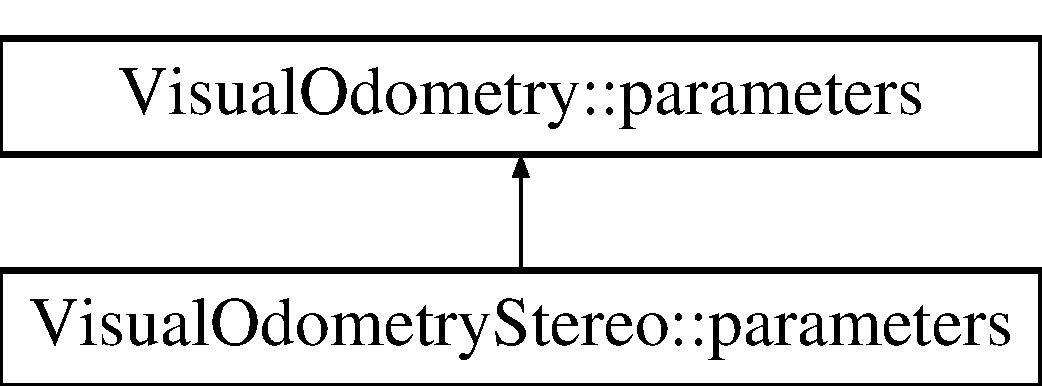
\includegraphics[height=2.000000cm]{struct_visual_odometry_stereo_1_1parameters}
\end{center}
\end{figure}
\subsection*{Public Attributes}
\begin{DoxyCompactItemize}
\item 
\hypertarget{struct_visual_odometry_stereo_1_1parameters_a94fac7929d0e5b260b72c0b57f838442}{double {\bfseries base}}\label{struct_visual_odometry_stereo_1_1parameters_a94fac7929d0e5b260b72c0b57f838442}

\item 
\hypertarget{struct_visual_odometry_stereo_1_1parameters_aefa853196599b4edb25b7f7fc722e938}{int32\+\_\+t {\bfseries ransac\+\_\+iters}}\label{struct_visual_odometry_stereo_1_1parameters_aefa853196599b4edb25b7f7fc722e938}

\item 
\hypertarget{struct_visual_odometry_stereo_1_1parameters_a55acc43c6570ef1d76abd7a69cc2e0fe}{double {\bfseries inlier\+\_\+threshold}}\label{struct_visual_odometry_stereo_1_1parameters_a55acc43c6570ef1d76abd7a69cc2e0fe}

\item 
\hypertarget{struct_visual_odometry_stereo_1_1parameters_ac17f9b3c1ed1480f57fb02c4eaf517f1}{bool {\bfseries reweighting}}\label{struct_visual_odometry_stereo_1_1parameters_ac17f9b3c1ed1480f57fb02c4eaf517f1}

\end{DoxyCompactItemize}


The documentation for this struct was generated from the following file\+:\begin{DoxyCompactItemize}
\item 
libviso2/viso\+\_\+stereo.\+h\end{DoxyCompactItemize}

\hypertarget{struct_visual_odometry_1_1parameters}{\section{Visual\+Odometry\+:\+:parameters Struct Reference}
\label{struct_visual_odometry_1_1parameters}\index{Visual\+Odometry\+::parameters@{Visual\+Odometry\+::parameters}}
}
Inheritance diagram for Visual\+Odometry\+:\+:parameters\+:\begin{figure}[H]
\begin{center}
\leavevmode
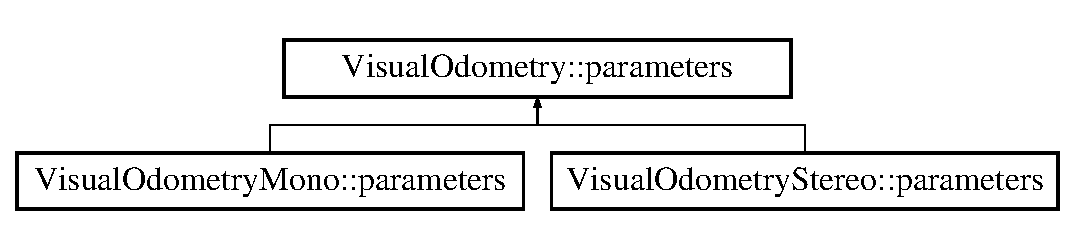
\includegraphics[height=2.000000cm]{struct_visual_odometry_1_1parameters}
\end{center}
\end{figure}
\subsection*{Public Attributes}
\begin{DoxyCompactItemize}
\item 
\hypertarget{struct_visual_odometry_1_1parameters_a6f734b57e08de115d0685f2d9aea7fa3}{\hyperlink{struct_matcher_1_1parameters}{Matcher\+::parameters} {\bfseries match}}\label{struct_visual_odometry_1_1parameters_a6f734b57e08de115d0685f2d9aea7fa3}

\item 
\hypertarget{struct_visual_odometry_1_1parameters_acc2eb54e9b22b1fdbdc83e7291b50d25}{\hyperlink{struct_visual_odometry_1_1bucketing}{Visual\+Odometry\+::bucketing} {\bfseries bucket}}\label{struct_visual_odometry_1_1parameters_acc2eb54e9b22b1fdbdc83e7291b50d25}

\item 
\hypertarget{struct_visual_odometry_1_1parameters_ad8fc3a97b88dc295c2dd1a8d027e2848}{\hyperlink{struct_visual_odometry_1_1calibration}{Visual\+Odometry\+::calibration} {\bfseries calib}}\label{struct_visual_odometry_1_1parameters_ad8fc3a97b88dc295c2dd1a8d027e2848}

\end{DoxyCompactItemize}


The documentation for this struct was generated from the following file\+:\begin{DoxyCompactItemize}
\item 
libviso2/viso.\+h\end{DoxyCompactItemize}

\hypertarget{struct_visual_odometry_mono_1_1parameters}{\section{Visual\+Odometry\+Mono\+:\+:parameters Struct Reference}
\label{struct_visual_odometry_mono_1_1parameters}\index{Visual\+Odometry\+Mono\+::parameters@{Visual\+Odometry\+Mono\+::parameters}}
}
Inheritance diagram for Visual\+Odometry\+Mono\+:\+:parameters\+:\begin{figure}[H]
\begin{center}
\leavevmode
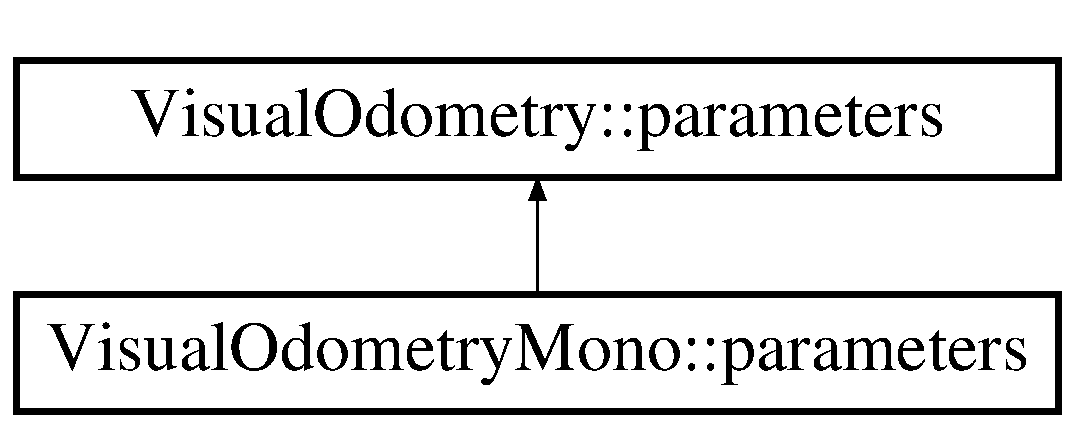
\includegraphics[height=2.000000cm]{struct_visual_odometry_mono_1_1parameters}
\end{center}
\end{figure}
\subsection*{Public Attributes}
\begin{DoxyCompactItemize}
\item 
\hypertarget{struct_visual_odometry_mono_1_1parameters_a9ef9008e32754fa03aaf29843879830b}{double {\bfseries height}}\label{struct_visual_odometry_mono_1_1parameters_a9ef9008e32754fa03aaf29843879830b}

\item 
\hypertarget{struct_visual_odometry_mono_1_1parameters_a6686713a1434bf1888a68583a4aaac3a}{double {\bfseries pitch}}\label{struct_visual_odometry_mono_1_1parameters_a6686713a1434bf1888a68583a4aaac3a}

\item 
\hypertarget{struct_visual_odometry_mono_1_1parameters_ac1c6895ee3e89c4d1e92d4ac5e5479d8}{int32\+\_\+t {\bfseries ransac\+\_\+iters}}\label{struct_visual_odometry_mono_1_1parameters_ac1c6895ee3e89c4d1e92d4ac5e5479d8}

\item 
\hypertarget{struct_visual_odometry_mono_1_1parameters_ac15db7ddbc967dabbbc724079bbe0a7b}{double {\bfseries inlier\+\_\+threshold}}\label{struct_visual_odometry_mono_1_1parameters_ac15db7ddbc967dabbbc724079bbe0a7b}

\item 
\hypertarget{struct_visual_odometry_mono_1_1parameters_a9a9ba628170a5c2bce117ea81f1c8a00}{double {\bfseries motion\+\_\+threshold}}\label{struct_visual_odometry_mono_1_1parameters_a9a9ba628170a5c2bce117ea81f1c8a00}

\end{DoxyCompactItemize}


The documentation for this struct was generated from the following file\+:\begin{DoxyCompactItemize}
\item 
libviso2/viso\+\_\+mono.\+h\end{DoxyCompactItemize}

\hypertarget{struct_matcher_1_1parameters}{\section{Matcher\+:\+:parameters Struct Reference}
\label{struct_matcher_1_1parameters}\index{Matcher\+::parameters@{Matcher\+::parameters}}
}
\subsection*{Public Attributes}
\begin{DoxyCompactItemize}
\item 
\hypertarget{struct_matcher_1_1parameters_a9820e6e263d60c483af5841d13098401}{int32\+\_\+t {\bfseries nms\+\_\+n}}\label{struct_matcher_1_1parameters_a9820e6e263d60c483af5841d13098401}

\item 
\hypertarget{struct_matcher_1_1parameters_a16b40f28d3bf50ae8a7a83975fa14c07}{int32\+\_\+t {\bfseries nms\+\_\+tau}}\label{struct_matcher_1_1parameters_a16b40f28d3bf50ae8a7a83975fa14c07}

\item 
\hypertarget{struct_matcher_1_1parameters_a48379ecc77592481cd6d00af670b59bb}{int32\+\_\+t {\bfseries match\+\_\+binsize}}\label{struct_matcher_1_1parameters_a48379ecc77592481cd6d00af670b59bb}

\item 
\hypertarget{struct_matcher_1_1parameters_a16a9accda09c16eb650a1b2b7a629625}{int32\+\_\+t {\bfseries match\+\_\+radius}}\label{struct_matcher_1_1parameters_a16a9accda09c16eb650a1b2b7a629625}

\item 
\hypertarget{struct_matcher_1_1parameters_a5166550b921eface419dbf8470c2aec4}{int32\+\_\+t {\bfseries match\+\_\+disp\+\_\+tolerance}}\label{struct_matcher_1_1parameters_a5166550b921eface419dbf8470c2aec4}

\item 
\hypertarget{struct_matcher_1_1parameters_a0595f0b135ef4aa2dbf41b5327c35da5}{int32\+\_\+t {\bfseries outlier\+\_\+disp\+\_\+tolerance}}\label{struct_matcher_1_1parameters_a0595f0b135ef4aa2dbf41b5327c35da5}

\item 
\hypertarget{struct_matcher_1_1parameters_afc412d3892d9a58ce9594dd0156e084d}{int32\+\_\+t {\bfseries outlier\+\_\+flow\+\_\+tolerance}}\label{struct_matcher_1_1parameters_afc412d3892d9a58ce9594dd0156e084d}

\item 
\hypertarget{struct_matcher_1_1parameters_a62fe233d2ac12916133be544ec85f763}{int32\+\_\+t {\bfseries multi\+\_\+stage}}\label{struct_matcher_1_1parameters_a62fe233d2ac12916133be544ec85f763}

\item 
\hypertarget{struct_matcher_1_1parameters_a4eb0242decd2f4b2bfd44660247b97cc}{int32\+\_\+t {\bfseries half\+\_\+resolution}}\label{struct_matcher_1_1parameters_a4eb0242decd2f4b2bfd44660247b97cc}

\item 
\hypertarget{struct_matcher_1_1parameters_ad3843c72dd15e8782fad2c169213fe8f}{int32\+\_\+t {\bfseries refinement}}\label{struct_matcher_1_1parameters_ad3843c72dd15e8782fad2c169213fe8f}

\item 
\hypertarget{struct_matcher_1_1parameters_a2dd27d4180b2fd7f761c35e44d5b3d54}{double {\bfseries f}}\label{struct_matcher_1_1parameters_a2dd27d4180b2fd7f761c35e44d5b3d54}

\item 
\hypertarget{struct_matcher_1_1parameters_ad66254c652eef7b857be5b524f2a5d5c}{double {\bfseries cu}}\label{struct_matcher_1_1parameters_ad66254c652eef7b857be5b524f2a5d5c}

\item 
\hypertarget{struct_matcher_1_1parameters_ab8c0a32ab52a943a1bbcb720528dd3ab}{double {\bfseries cv}}\label{struct_matcher_1_1parameters_ab8c0a32ab52a943a1bbcb720528dd3ab}

\item 
\hypertarget{struct_matcher_1_1parameters_a54fd8ef17d17d69591a0822a7d77ee7e}{double {\bfseries base}}\label{struct_matcher_1_1parameters_a54fd8ef17d17d69591a0822a7d77ee7e}

\end{DoxyCompactItemize}


The documentation for this struct was generated from the following file\+:\begin{DoxyCompactItemize}
\item 
libviso2/matcher.\+h\end{DoxyCompactItemize}

\hypertarget{struct_reconstruction_1_1point3d}{\section{Reconstruction\+:\+:point3d Struct Reference}
\label{struct_reconstruction_1_1point3d}\index{Reconstruction\+::point3d@{Reconstruction\+::point3d}}
}
\subsection*{Public Member Functions}
\begin{DoxyCompactItemize}
\item 
\hypertarget{struct_reconstruction_1_1point3d_a67e779ec8a7df14e4c2a39533e0e10a2}{{\bfseries point3d} (float x, float y, float z)}\label{struct_reconstruction_1_1point3d_a67e779ec8a7df14e4c2a39533e0e10a2}

\end{DoxyCompactItemize}
\subsection*{Public Attributes}
\begin{DoxyCompactItemize}
\item 
\hypertarget{struct_reconstruction_1_1point3d_ab66110baf26112dceb5bdfe196d4cfac}{float {\bfseries x}}\label{struct_reconstruction_1_1point3d_ab66110baf26112dceb5bdfe196d4cfac}

\item 
\hypertarget{struct_reconstruction_1_1point3d_a8babfa0adf6b84bb79d99df88055461f}{float {\bfseries y}}\label{struct_reconstruction_1_1point3d_a8babfa0adf6b84bb79d99df88055461f}

\item 
\hypertarget{struct_reconstruction_1_1point3d_aa0eaffb29c824544bcd9785cc9e9b8cc}{float {\bfseries z}}\label{struct_reconstruction_1_1point3d_aa0eaffb29c824544bcd9785cc9e9b8cc}

\end{DoxyCompactItemize}


The documentation for this struct was generated from the following file\+:\begin{DoxyCompactItemize}
\item 
libviso2/reconstruction.\+h\end{DoxyCompactItemize}

\hypertarget{class_reconstruction}{\section{Reconstruction Class Reference}
\label{class_reconstruction}\index{Reconstruction@{Reconstruction}}
}
\subsection*{Classes}
\begin{DoxyCompactItemize}
\item 
struct \hyperlink{struct_reconstruction_1_1point3d}{point3d}
\end{DoxyCompactItemize}
\subsection*{Public Member Functions}
\begin{DoxyCompactItemize}
\item 
\hypertarget{class_reconstruction_ab76af4a64c0be541da68775d033e0dc3}{void {\bfseries set\+Calibration} (F\+L\+O\+A\+T f, F\+L\+O\+A\+T cu, F\+L\+O\+A\+T cv)}\label{class_reconstruction_ab76af4a64c0be541da68775d033e0dc3}

\item 
\hypertarget{class_reconstruction_a206232fe226bcea650239aa42369e557}{void {\bfseries update} (std\+::vector$<$ \hyperlink{struct_matcher_1_1p__match}{Matcher\+::p\+\_\+match} $>$ p\+\_\+matched, \hyperlink{class_matrix}{Matrix} Tr, int32\+\_\+t point\+\_\+type=1, int32\+\_\+t min\+\_\+track\+\_\+length=2, double max\+\_\+dist=30, double min\+\_\+angle=2)}\label{class_reconstruction_a206232fe226bcea650239aa42369e557}

\item 
\hypertarget{class_reconstruction_a32a376c7c0a79628a15ed9184edc4a3e}{std\+::vector$<$ \hyperlink{struct_reconstruction_1_1point3d}{point3d} $>$ {\bfseries get\+Points} ()}\label{class_reconstruction_a32a376c7c0a79628a15ed9184edc4a3e}

\end{DoxyCompactItemize}


The documentation for this class was generated from the following files\+:\begin{DoxyCompactItemize}
\item 
libviso2/reconstruction.\+h\item 
libviso2/reconstruction.\+cpp\end{DoxyCompactItemize}

\hypertarget{structsplaynode}{\section{splaynode Struct Reference}
\label{structsplaynode}\index{splaynode@{splaynode}}
}
\subsection*{Public Attributes}
\begin{DoxyCompactItemize}
\item 
\hypertarget{structsplaynode_aaa9fc6e2d568c0be2a5a4c0831965c4f}{struct \hyperlink{structotri}{otri} {\bfseries keyedge}}\label{structsplaynode_aaa9fc6e2d568c0be2a5a4c0831965c4f}

\item 
\hypertarget{structsplaynode_a63438aac02b8993141ebf848c347098d}{vertex {\bfseries keydest}}\label{structsplaynode_a63438aac02b8993141ebf848c347098d}

\item 
\hypertarget{structsplaynode_a67b52cb89e958acbdf9761ea4aab6813}{struct \hyperlink{structsplaynode}{splaynode} $\ast$ {\bfseries lchild}}\label{structsplaynode_a67b52cb89e958acbdf9761ea4aab6813}

\item 
\hypertarget{structsplaynode_ac1cf5f799931eda1315037dc7d0bce3a}{struct \hyperlink{structsplaynode}{splaynode} $\ast$ {\bfseries rchild}}\label{structsplaynode_ac1cf5f799931eda1315037dc7d0bce3a}

\end{DoxyCompactItemize}


The documentation for this struct was generated from the following file\+:\begin{DoxyCompactItemize}
\item 
libviso2/triangle.\+cpp\end{DoxyCompactItemize}

\hypertarget{class_timer}{\section{Timer Class Reference}
\label{class_timer}\index{Timer@{Timer}}
}
\subsection*{Public Member Functions}
\begin{DoxyCompactItemize}
\item 
\hypertarget{class_timer_a483491cfb75be6f7466c5637a602b54f}{void {\bfseries start} (std\+::string title)}\label{class_timer_a483491cfb75be6f7466c5637a602b54f}

\item 
\hypertarget{class_timer_a63f0eb44b27402196590a03781515dba}{void {\bfseries stop} ()}\label{class_timer_a63f0eb44b27402196590a03781515dba}

\item 
\hypertarget{class_timer_a882129bf76094abcd8972c9d3855359c}{void {\bfseries plot} ()}\label{class_timer_a882129bf76094abcd8972c9d3855359c}

\item 
\hypertarget{class_timer_a9020542d73357a4eef512eefaf57524b}{void {\bfseries reset} ()}\label{class_timer_a9020542d73357a4eef512eefaf57524b}

\end{DoxyCompactItemize}


The documentation for this class was generated from the following file\+:\begin{DoxyCompactItemize}
\item 
libviso2/timer.\+h\end{DoxyCompactItemize}

\hypertarget{structtriangulateio}{\section{triangulateio Struct Reference}
\label{structtriangulateio}\index{triangulateio@{triangulateio}}
}
\subsection*{Public Attributes}
\begin{DoxyCompactItemize}
\item 
\hypertarget{structtriangulateio_a82a64e7bbed8533faa445851f3d2e915}{float $\ast$ {\bfseries pointlist}}\label{structtriangulateio_a82a64e7bbed8533faa445851f3d2e915}

\item 
\hypertarget{structtriangulateio_ae2d48c6a745b2fb93430beb287373469}{float $\ast$ {\bfseries pointattributelist}}\label{structtriangulateio_ae2d48c6a745b2fb93430beb287373469}

\item 
\hypertarget{structtriangulateio_acb2a9792412a2c3051fb869e88cfa602}{int $\ast$ {\bfseries pointmarkerlist}}\label{structtriangulateio_acb2a9792412a2c3051fb869e88cfa602}

\item 
\hypertarget{structtriangulateio_a29be46ad3fc4f8c84235e420f7e606ec}{int {\bfseries numberofpoints}}\label{structtriangulateio_a29be46ad3fc4f8c84235e420f7e606ec}

\item 
\hypertarget{structtriangulateio_aaac6a34f7d7bf1d1476ce7672f15d976}{int {\bfseries numberofpointattributes}}\label{structtriangulateio_aaac6a34f7d7bf1d1476ce7672f15d976}

\item 
\hypertarget{structtriangulateio_a7d0f1c11cd6dc624ae61dbbbcc68b8cb}{int $\ast$ {\bfseries trianglelist}}\label{structtriangulateio_a7d0f1c11cd6dc624ae61dbbbcc68b8cb}

\item 
\hypertarget{structtriangulateio_a308a628907c92aff9d23da64895cf786}{float $\ast$ {\bfseries triangleattributelist}}\label{structtriangulateio_a308a628907c92aff9d23da64895cf786}

\item 
\hypertarget{structtriangulateio_ad05a9d4c4941dbdb8193cfedb289963a}{float $\ast$ {\bfseries trianglearealist}}\label{structtriangulateio_ad05a9d4c4941dbdb8193cfedb289963a}

\item 
\hypertarget{structtriangulateio_a266c62c74f443a4a50c986ccf97e74c7}{int $\ast$ {\bfseries neighborlist}}\label{structtriangulateio_a266c62c74f443a4a50c986ccf97e74c7}

\item 
\hypertarget{structtriangulateio_a6455c22dba63bdb0584d44fdf35a321f}{int {\bfseries numberoftriangles}}\label{structtriangulateio_a6455c22dba63bdb0584d44fdf35a321f}

\item 
\hypertarget{structtriangulateio_aaeeda011ca1f51696fcc5a460b81c18d}{int {\bfseries numberofcorners}}\label{structtriangulateio_aaeeda011ca1f51696fcc5a460b81c18d}

\item 
\hypertarget{structtriangulateio_a272ba3b8730997b1bd6c367328b1abf8}{int {\bfseries numberoftriangleattributes}}\label{structtriangulateio_a272ba3b8730997b1bd6c367328b1abf8}

\item 
\hypertarget{structtriangulateio_ad45fec0a70058760450e09b949a3d1c0}{int $\ast$ {\bfseries segmentlist}}\label{structtriangulateio_ad45fec0a70058760450e09b949a3d1c0}

\item 
\hypertarget{structtriangulateio_a8d88affa03ad1156b1d087448166bf04}{int $\ast$ {\bfseries segmentmarkerlist}}\label{structtriangulateio_a8d88affa03ad1156b1d087448166bf04}

\item 
\hypertarget{structtriangulateio_a417da9cc4711390560c6af7750d13d95}{int {\bfseries numberofsegments}}\label{structtriangulateio_a417da9cc4711390560c6af7750d13d95}

\item 
\hypertarget{structtriangulateio_a825d0bf2619c98fea6aa9f456dc53077}{float $\ast$ {\bfseries holelist}}\label{structtriangulateio_a825d0bf2619c98fea6aa9f456dc53077}

\item 
\hypertarget{structtriangulateio_a91deb1af3dd2ef937f1b6b7e38261e99}{int {\bfseries numberofholes}}\label{structtriangulateio_a91deb1af3dd2ef937f1b6b7e38261e99}

\item 
\hypertarget{structtriangulateio_ac0dde436bb3933efdf64a3980e4917f1}{float $\ast$ {\bfseries regionlist}}\label{structtriangulateio_ac0dde436bb3933efdf64a3980e4917f1}

\item 
\hypertarget{structtriangulateio_ac1082ccae35526598ba0977068da9278}{int {\bfseries numberofregions}}\label{structtriangulateio_ac1082ccae35526598ba0977068da9278}

\item 
\hypertarget{structtriangulateio_af8374f90431a318b694bb5424814f111}{int $\ast$ {\bfseries edgelist}}\label{structtriangulateio_af8374f90431a318b694bb5424814f111}

\item 
\hypertarget{structtriangulateio_a3f9be953734099d409f54736c3cd72af}{int $\ast$ {\bfseries edgemarkerlist}}\label{structtriangulateio_a3f9be953734099d409f54736c3cd72af}

\item 
\hypertarget{structtriangulateio_ad47e80dd7941e0693335c9a512746b38}{float $\ast$ {\bfseries normlist}}\label{structtriangulateio_ad47e80dd7941e0693335c9a512746b38}

\item 
\hypertarget{structtriangulateio_ac8c1b394861ed4a5c021a2d08a36a2a9}{int {\bfseries numberofedges}}\label{structtriangulateio_ac8c1b394861ed4a5c021a2d08a36a2a9}

\end{DoxyCompactItemize}


The documentation for this struct was generated from the following file\+:\begin{DoxyCompactItemize}
\item 
libviso2/triangle.\+h\end{DoxyCompactItemize}

\hypertarget{class_visual_odometry}{\section{Visual\+Odometry Class Reference}
\label{class_visual_odometry}\index{Visual\+Odometry@{Visual\+Odometry}}
}
Inheritance diagram for Visual\+Odometry\+:\begin{figure}[H]
\begin{center}
\leavevmode
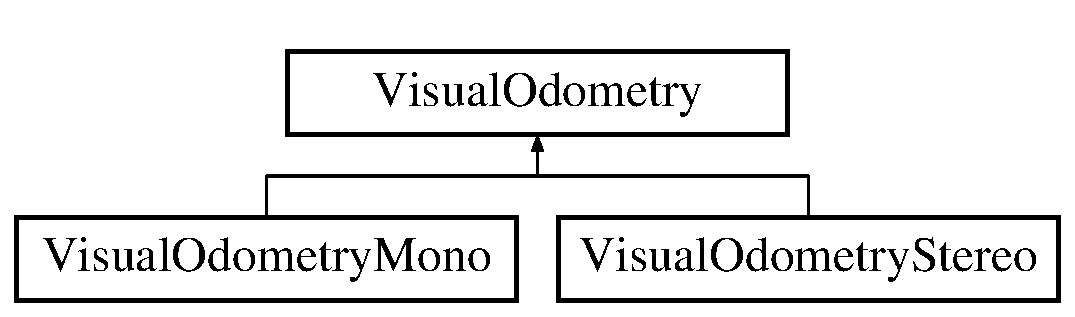
\includegraphics[height=2.000000cm]{class_visual_odometry}
\end{center}
\end{figure}
\subsection*{Classes}
\begin{DoxyCompactItemize}
\item 
struct \hyperlink{struct_visual_odometry_1_1bucketing}{bucketing}
\item 
struct \hyperlink{struct_visual_odometry_1_1calibration}{calibration}
\item 
struct \hyperlink{struct_visual_odometry_1_1parameters}{parameters}
\end{DoxyCompactItemize}
\subsection*{Public Member Functions}
\begin{DoxyCompactItemize}
\item 
\hypertarget{class_visual_odometry_aca4e1f1cc799f6392303ab7fca26f81e}{{\bfseries Visual\+Odometry} (\hyperlink{struct_visual_odometry_1_1parameters}{parameters} param)}\label{class_visual_odometry_aca4e1f1cc799f6392303ab7fca26f81e}

\item 
\hypertarget{class_visual_odometry_af386ca261ddfc82c1da66cc92fb8554c}{bool {\bfseries process} (std\+::vector$<$ \hyperlink{struct_matcher_1_1p__match}{Matcher\+::p\+\_\+match} $>$ p\+\_\+matched\+\_\+)}\label{class_visual_odometry_af386ca261ddfc82c1da66cc92fb8554c}

\item 
\hypertarget{class_visual_odometry_a0e25df50775b1d6ccf65cfb582fcec6c}{\hyperlink{class_matrix}{Matrix} {\bfseries get\+Motion} ()}\label{class_visual_odometry_a0e25df50775b1d6ccf65cfb582fcec6c}

\item 
\hypertarget{class_visual_odometry_a3188ba4cd672fe3af210485b2234dfda}{std\+::vector$<$ \hyperlink{struct_matcher_1_1p__match}{Matcher\+::p\+\_\+match} $>$ {\bfseries get\+Matches} ()}\label{class_visual_odometry_a3188ba4cd672fe3af210485b2234dfda}

\item 
\hypertarget{class_visual_odometry_a5cdf9079cd4f96e782c15c97893af186}{int32\+\_\+t {\bfseries get\+Number\+Of\+Matches} ()}\label{class_visual_odometry_a5cdf9079cd4f96e782c15c97893af186}

\item 
\hypertarget{class_visual_odometry_a59dd3aec4cd992069eee7903621cef6a}{int32\+\_\+t {\bfseries get\+Number\+Of\+Inliers} ()}\label{class_visual_odometry_a59dd3aec4cd992069eee7903621cef6a}

\item 
\hypertarget{class_visual_odometry_a7ffc656cdb1d695a5981b44806749bde}{std\+::vector$<$ int32\+\_\+t $>$ {\bfseries get\+Inlier\+Indices} ()}\label{class_visual_odometry_a7ffc656cdb1d695a5981b44806749bde}

\item 
\hypertarget{class_visual_odometry_a3968f4e85ee9b06986a37a9430f899ab}{float {\bfseries get\+Gain} (std\+::vector$<$ int32\+\_\+t $>$ inliers\+\_\+)}\label{class_visual_odometry_a3968f4e85ee9b06986a37a9430f899ab}

\end{DoxyCompactItemize}
\subsection*{Protected Member Functions}
\begin{DoxyCompactItemize}
\item 
\hypertarget{class_visual_odometry_a9caa39c2a95ede9ee423a60c49781324}{bool {\bfseries update\+Motion} ()}\label{class_visual_odometry_a9caa39c2a95ede9ee423a60c49781324}

\item 
\hypertarget{class_visual_odometry_af98bab368513d4c69a6e49f5f3220dc8}{\hyperlink{class_matrix}{Matrix} {\bfseries transformation\+Vector\+To\+Matrix} (std\+::vector$<$ double $>$ tr)}\label{class_visual_odometry_af98bab368513d4c69a6e49f5f3220dc8}

\item 
\hypertarget{class_visual_odometry_a744ce1154259dcf50a4632c1da93310b}{virtual std\+::vector$<$ double $>$ {\bfseries estimate\+Motion} (std\+::vector$<$ \hyperlink{struct_matcher_1_1p__match}{Matcher\+::p\+\_\+match} $>$ p\+\_\+matched)=0}\label{class_visual_odometry_a744ce1154259dcf50a4632c1da93310b}

\item 
\hypertarget{class_visual_odometry_a2d416460beaa8ef87cb5d9ce45ce25b2}{std\+::vector$<$ int32\+\_\+t $>$ {\bfseries get\+Random\+Sample} (int32\+\_\+t N, int32\+\_\+t num)}\label{class_visual_odometry_a2d416460beaa8ef87cb5d9ce45ce25b2}

\end{DoxyCompactItemize}
\subsection*{Protected Attributes}
\begin{DoxyCompactItemize}
\item 
\hypertarget{class_visual_odometry_ae4d1f67aa13d39d4e2d79b66c24d40cd}{\hyperlink{class_matrix}{Matrix} {\bfseries Tr\+\_\+delta}}\label{class_visual_odometry_ae4d1f67aa13d39d4e2d79b66c24d40cd}

\item 
\hypertarget{class_visual_odometry_a7adb170f1f42afc4af02967fa59d5bd4}{bool {\bfseries Tr\+\_\+valid}}\label{class_visual_odometry_a7adb170f1f42afc4af02967fa59d5bd4}

\item 
\hypertarget{class_visual_odometry_acad7f354f64ac9c31ffdca21ad4a81ea}{\hyperlink{class_matcher}{Matcher} $\ast$ {\bfseries matcher}}\label{class_visual_odometry_acad7f354f64ac9c31ffdca21ad4a81ea}

\item 
\hypertarget{class_visual_odometry_a90a6b44dea99f73af1becbec27f574dc}{std\+::vector$<$ int32\+\_\+t $>$ {\bfseries inliers}}\label{class_visual_odometry_a90a6b44dea99f73af1becbec27f574dc}

\item 
\hypertarget{class_visual_odometry_a460b88e3c6413862891cdac83c5f013d}{double $\ast$ {\bfseries J}}\label{class_visual_odometry_a460b88e3c6413862891cdac83c5f013d}

\item 
\hypertarget{class_visual_odometry_a48bbbc977f2de8bb647842a9a14fed34}{double $\ast$ {\bfseries p\+\_\+observe}}\label{class_visual_odometry_a48bbbc977f2de8bb647842a9a14fed34}

\item 
\hypertarget{class_visual_odometry_a58bee4df50653cd9b7de41f7c0b53280}{double $\ast$ {\bfseries p\+\_\+predict}}\label{class_visual_odometry_a58bee4df50653cd9b7de41f7c0b53280}

\item 
\hypertarget{class_visual_odometry_a80f624e6d5e587d972c3e69781321ed0}{std\+::vector$<$ \hyperlink{struct_matcher_1_1p__match}{Matcher\+::p\+\_\+match} $>$ {\bfseries p\+\_\+matched}}\label{class_visual_odometry_a80f624e6d5e587d972c3e69781321ed0}

\end{DoxyCompactItemize}
\subsection*{Friends}
\begin{DoxyCompactItemize}
\item 
\hypertarget{class_visual_odometry_a46e1f3711d18286d269160ee44217306}{std\+::ostream \& {\bfseries operator$<$$<$} (std\+::ostream \&os, \hyperlink{class_visual_odometry}{Visual\+Odometry} \&viso)}\label{class_visual_odometry_a46e1f3711d18286d269160ee44217306}

\end{DoxyCompactItemize}


The documentation for this class was generated from the following files\+:\begin{DoxyCompactItemize}
\item 
libviso2/viso.\+h\item 
libviso2/viso.\+cpp\end{DoxyCompactItemize}

\hypertarget{class_visual_odometry_mono}{\section{Visual\+Odometry\+Mono Class Reference}
\label{class_visual_odometry_mono}\index{Visual\+Odometry\+Mono@{Visual\+Odometry\+Mono}}
}
Inheritance diagram for Visual\+Odometry\+Mono\+:\begin{figure}[H]
\begin{center}
\leavevmode
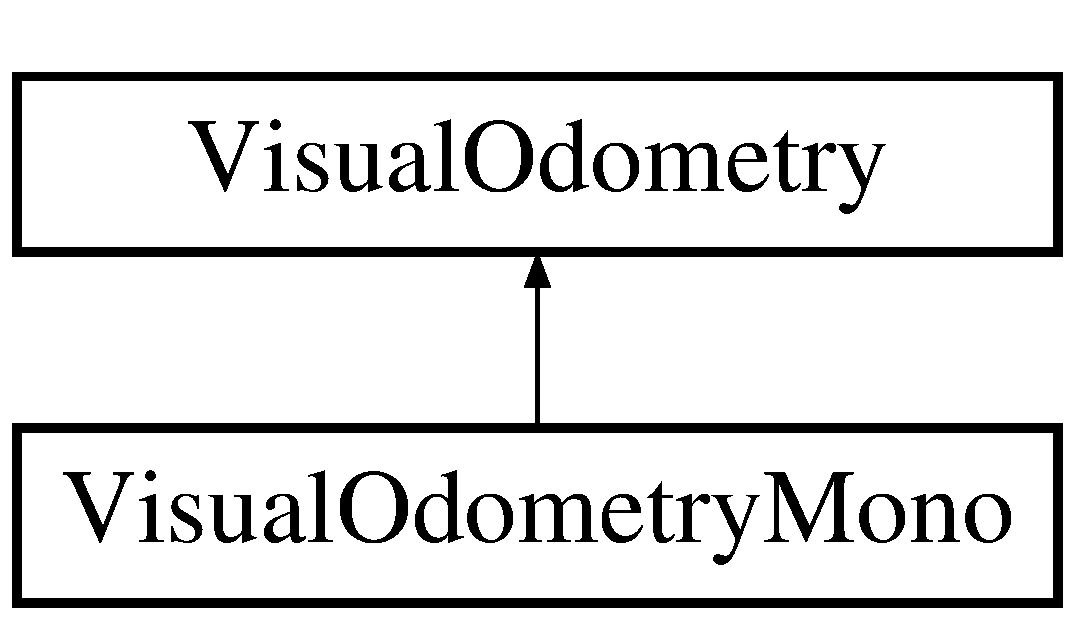
\includegraphics[height=2.000000cm]{class_visual_odometry_mono}
\end{center}
\end{figure}
\subsection*{Classes}
\begin{DoxyCompactItemize}
\item 
struct \hyperlink{struct_visual_odometry_mono_1_1parameters}{parameters}
\end{DoxyCompactItemize}
\subsection*{Public Member Functions}
\begin{DoxyCompactItemize}
\item 
\hypertarget{class_visual_odometry_mono_af4d9e82b3e369a8896192068c673e47a}{{\bfseries Visual\+Odometry\+Mono} (\hyperlink{struct_visual_odometry_mono_1_1parameters}{parameters} param)}\label{class_visual_odometry_mono_af4d9e82b3e369a8896192068c673e47a}

\item 
\hypertarget{class_visual_odometry_mono_a450a424f898de00b5441ad0c0931d38c}{bool {\bfseries process} (uint8\+\_\+t $\ast$I, int32\+\_\+t $\ast$dims, bool replace=false)}\label{class_visual_odometry_mono_a450a424f898de00b5441ad0c0931d38c}

\end{DoxyCompactItemize}
\subsection*{Additional Inherited Members}


The documentation for this class was generated from the following files\+:\begin{DoxyCompactItemize}
\item 
libviso2/viso\+\_\+mono.\+h\item 
libviso2/viso\+\_\+mono.\+cpp\end{DoxyCompactItemize}

\hypertarget{class_visual_odometry_stereo}{\section{Visual\+Odometry\+Stereo Class Reference}
\label{class_visual_odometry_stereo}\index{Visual\+Odometry\+Stereo@{Visual\+Odometry\+Stereo}}
}
Inheritance diagram for Visual\+Odometry\+Stereo\+:\begin{figure}[H]
\begin{center}
\leavevmode
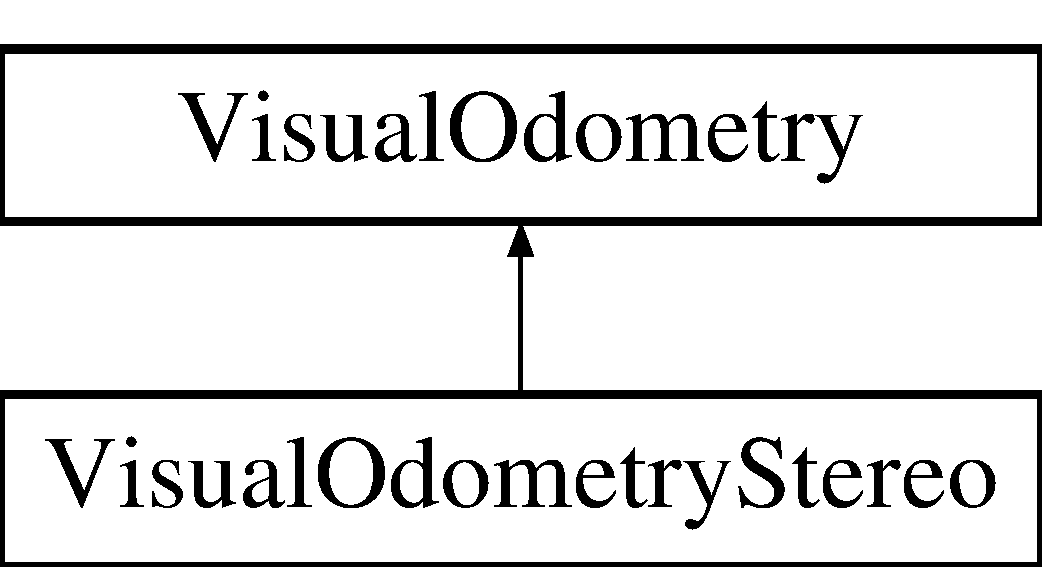
\includegraphics[height=2.000000cm]{class_visual_odometry_stereo}
\end{center}
\end{figure}
\subsection*{Classes}
\begin{DoxyCompactItemize}
\item 
struct \hyperlink{struct_visual_odometry_stereo_1_1parameters}{parameters}
\end{DoxyCompactItemize}
\subsection*{Public Member Functions}
\begin{DoxyCompactItemize}
\item 
\hypertarget{class_visual_odometry_stereo_ae77d23d33e9782c89d507a77f08df779}{{\bfseries Visual\+Odometry\+Stereo} (\hyperlink{struct_visual_odometry_stereo_1_1parameters}{parameters} param)}\label{class_visual_odometry_stereo_ae77d23d33e9782c89d507a77f08df779}

\item 
\hypertarget{class_visual_odometry_stereo_aa9832cd5fe9bc352418803f442c450a6}{bool {\bfseries process} (uint8\+\_\+t $\ast$I1, uint8\+\_\+t $\ast$I2, int32\+\_\+t $\ast$dims, bool replace=false)}\label{class_visual_odometry_stereo_aa9832cd5fe9bc352418803f442c450a6}

\end{DoxyCompactItemize}
\subsection*{Additional Inherited Members}


The documentation for this class was generated from the following files\+:\begin{DoxyCompactItemize}
\item 
libviso2/viso\+\_\+stereo.\+h\item 
libviso2/viso\+\_\+stereo.\+cpp\end{DoxyCompactItemize}

%--- End generated contents ---

% Index
\newpage
\phantomsection
\addcontentsline{toc}{chapter}{Index}
\printindex

\end{document}
